\documentclass[1p]{elsarticle_modified}
%\bibliographystyle{elsarticle-num}

%\usepackage[colorlinks]{hyperref}
%\usepackage{abbrmath_seonhwa} %\Abb, \Ascr, \Acal ,\Abf, \Afrak
\usepackage{amsfonts}
\usepackage{amssymb}
\usepackage{amsmath}
\usepackage{amsthm}
\usepackage{scalefnt}
\usepackage{amsbsy}
\usepackage{kotex}
\usepackage{caption}
\usepackage{subfig}
\usepackage{color}
\usepackage{graphicx}
\usepackage{xcolor} %% white, black, red, green, blue, cyan, magenta, yellow
\usepackage{float}
\usepackage{setspace}
\usepackage{hyperref}

\usepackage{tikz}
\usetikzlibrary{arrows}

\usepackage{multirow}
\usepackage{array} % fixed length table
\usepackage{hhline}

%%%%%%%%%%%%%%%%%%%%%
\makeatletter
\renewcommand*\env@matrix[1][\arraystretch]{%
	\edef\arraystretch{#1}%
	\hskip -\arraycolsep
	\let\@ifnextchar\new@ifnextchar
	\array{*\c@MaxMatrixCols c}}
\makeatother %https://tex.stackexchange.com/questions/14071/how-can-i-increase-the-line-spacing-in-a-matrix
%%%%%%%%%%%%%%%

\usepackage[normalem]{ulem}

\newcommand{\msout}[1]{\ifmmode\text{\sout{\ensuremath{#1}}}\else\sout{#1}\fi}
%SOURCE: \msout is \stkout macro in https://tex.stackexchange.com/questions/20609/strikeout-in-math-mode

\newcommand{\cancel}[1]{
	\ifmmode
	{\color{red}\msout{#1}}
	\else
	{\color{red}\sout{#1}}
	\fi
}

\newcommand{\add}[1]{
	{\color{blue}\uwave{#1}}
}

\newcommand{\replace}[2]{
	\ifmmode
	{\color{red}\msout{#1}}{\color{blue}\uwave{#2}}
	\else
	{\color{red}\sout{#1}}{\color{blue}\uwave{#2}}
	\fi
}

\newcommand{\Sol}{\mathcal{S}} %segment
\newcommand{\D}{D} %diagram
\newcommand{\A}{\mathcal{A}} %arc


%%%%%%%%%%%%%%%%%%%%%%%%%%%%%5 test

\def\sl{\operatorname{\textup{SL}}(2,\Cbb)}
\def\psl{\operatorname{\textup{PSL}}(2,\Cbb)}
\def\quan{\mkern 1mu \triangleright \mkern 1mu}

\theoremstyle{definition}
\newtheorem{thm}{Theorem}[section]
\newtheorem{prop}[thm]{Proposition}
\newtheorem{lem}[thm]{Lemma}
\newtheorem{ques}[thm]{Question}
\newtheorem{cor}[thm]{Corollary}
\newtheorem{defn}[thm]{Definition}
\newtheorem{exam}[thm]{Example}
\newtheorem{rmk}[thm]{Remark}
\newtheorem{alg}[thm]{Algorithm}

\newcommand{\I}{\sqrt{-1}}
\begin{document}

%\begin{frontmatter}
%
%\title{Boundary parabolic representations of knots up to 8 crossings}
%
%%% Group authors per affiliation:
%\author{Yunhi Cho} 
%\address{Department of Mathematics, University of Seoul, Seoul, Korea}
%\ead{yhcho@uos.ac.kr}
%
%
%\author{Seonhwa Kim} %\fnref{s_kim}}
%\address{Center for Geometry and Physics, Institute for Basic Science, Pohang, 37673, Korea}
%\ead{ryeona17@ibs.re.kr}
%
%\author{Hyuk Kim}
%\address{Department of Mathematical Sciences, Seoul National University, Seoul 08826, Korea}
%\ead{hyukkim@snu.ac.kr}
%
%\author{Seokbeom Yoon}
%\address{Department of Mathematical Sciences, Seoul National University, Seoul, 08826,  Korea}
%\ead{sbyoon15@snu.ac.kr}
%
%\begin{abstract}
%We find all boundary parabolic representation of knots up to 8 crossings.
%
%\end{abstract}
%\begin{keyword}
%    \MSC[2010] 57M25 
%\end{keyword}
%
%\end{frontmatter}

%\linenumbers
%\tableofcontents
%
\newcommand\colored[1]{\textcolor{white}{\rule[-0.35ex]{0.8em}{1.4ex}}\kern-0.8em\color{red} #1}%
%\newcommand\colored[1]{\textcolor{white}{ #1}\kern-2.17ex	\textcolor{white}{ #1}\kern-1.81ex	\textcolor{white}{ #1}\kern-2.15ex\color{red}#1	}

{\Large $\underline{12a_{0389}~(K12a_{0389})}$}

\setlength{\tabcolsep}{10pt}
\renewcommand{\arraystretch}{1.6}
\vspace{1cm}\begin{tabular}{m{100pt}>{\centering\arraybackslash}m{274pt}}
\multirow{5}{120pt}{
	\centering
	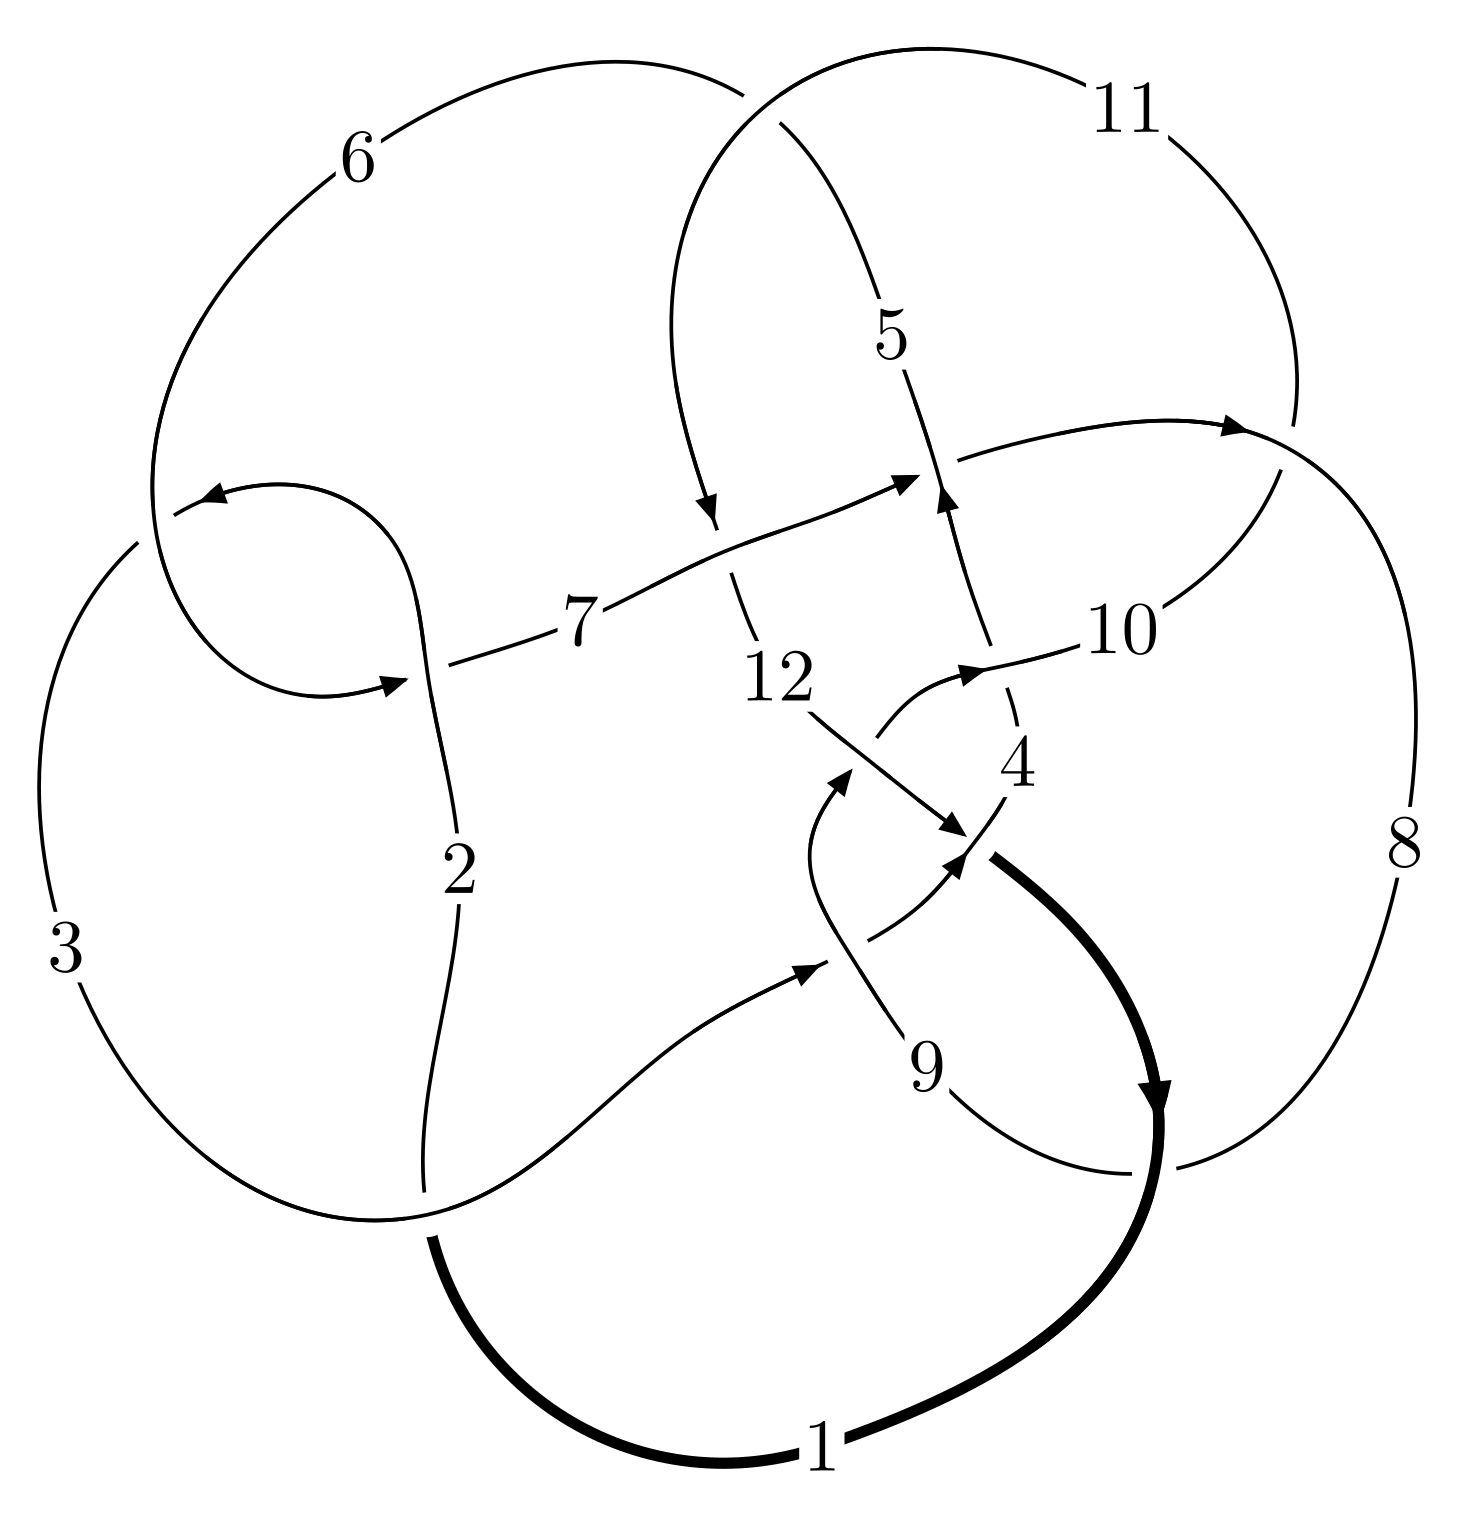
\includegraphics[width=112pt]{../../../GIT/diagram.site/Diagrams/png/1190_12a_0389.png}\\
\ \ \ A knot diagram\footnotemark}&
\allowdisplaybreaks
\textbf{Linearized knot diagam} \\
\cline{2-2}
 &
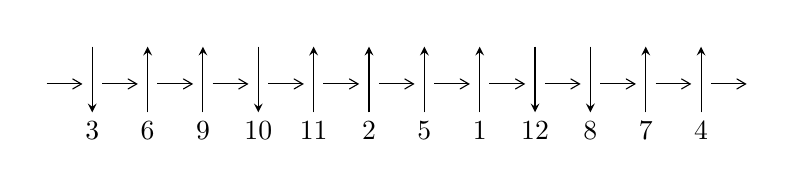
\begin{tikzpicture}[x=20pt, y=17pt]
	% nodes
	\node (C0) at (0, 0) {};
	\node (C1) at (1, 0) {};
	\node (C1U) at (1, +1) {};
	\node (C1D) at (1, -1) {3};

	\node (C2) at (2, 0) {};
	\node (C2U) at (2, +1) {};
	\node (C2D) at (2, -1) {6};

	\node (C3) at (3, 0) {};
	\node (C3U) at (3, +1) {};
	\node (C3D) at (3, -1) {9};

	\node (C4) at (4, 0) {};
	\node (C4U) at (4, +1) {};
	\node (C4D) at (4, -1) {10};

	\node (C5) at (5, 0) {};
	\node (C5U) at (5, +1) {};
	\node (C5D) at (5, -1) {11};

	\node (C6) at (6, 0) {};
	\node (C6U) at (6, +1) {};
	\node (C6D) at (6, -1) {2};

	\node (C7) at (7, 0) {};
	\node (C7U) at (7, +1) {};
	\node (C7D) at (7, -1) {5};

	\node (C8) at (8, 0) {};
	\node (C8U) at (8, +1) {};
	\node (C8D) at (8, -1) {1};

	\node (C9) at (9, 0) {};
	\node (C9U) at (9, +1) {};
	\node (C9D) at (9, -1) {12};

	\node (C10) at (10, 0) {};
	\node (C10U) at (10, +1) {};
	\node (C10D) at (10, -1) {8};

	\node (C11) at (11, 0) {};
	\node (C11U) at (11, +1) {};
	\node (C11D) at (11, -1) {7};

	\node (C12) at (12, 0) {};
	\node (C12U) at (12, +1) {};
	\node (C12D) at (12, -1) {4};
	\node (C13) at (13, 0) {};

	% arrows
	\draw[->,>={angle 60}]
	(C0) edge (C1) (C1) edge (C2) (C2) edge (C3) (C3) edge (C4) (C4) edge (C5) (C5) edge (C6) (C6) edge (C7) (C7) edge (C8) (C8) edge (C9) (C9) edge (C10) (C10) edge (C11) (C11) edge (C12) (C12) edge (C13) ;	\draw[->,>=stealth]
	(C1U) edge (C1D) (C2D) edge (C2U) (C3D) edge (C3U) (C4U) edge (C4D) (C5D) edge (C5U) (C6D) edge (C6U) (C7D) edge (C7U) (C8D) edge (C8U) (C9U) edge (C9D) (C10U) edge (C10D) (C11D) edge (C11U) (C12D) edge (C12U) ;
	\end{tikzpicture} \\
\hhline{~~} \\& 
\textbf{Solving Sequence} \\ \cline{2-2} 
 &
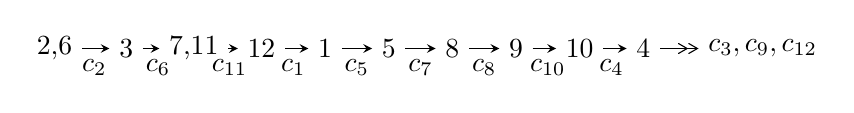
\begin{tikzpicture}[x=23pt, y=7pt]
	% node
	\node (A0) at (-1/8, 0) {2,6};
	\node (A1) at (1, 0) {3};
	\node (A2) at (33/16, 0) {7,11};
	\node (A3) at (25/8, 0) {12};
	\node (A4) at (33/8, 0) {1};
	\node (A5) at (41/8, 0) {5};
	\node (A6) at (49/8, 0) {8};
	\node (A7) at (57/8, 0) {9};
	\node (A8) at (65/8, 0) {10};
	\node (A9) at (73/8, 0) {4};
	\node (C1) at (1/2, -1) {$c_{2}$};
	\node (C2) at (3/2, -1) {$c_{6}$};
	\node (C3) at (21/8, -1) {$c_{11}$};
	\node (C4) at (29/8, -1) {$c_{1}$};
	\node (C5) at (37/8, -1) {$c_{5}$};
	\node (C6) at (45/8, -1) {$c_{7}$};
	\node (C7) at (53/8, -1) {$c_{8}$};
	\node (C8) at (61/8, -1) {$c_{10}$};
	\node (C9) at (69/8, -1) {$c_{4}$};
	\node (A10) at (11, 0) {$c_{3},c_{9},c_{12}$};

	% edge
	\draw[->,>=stealth]	
	(A0) edge (A1) (A1) edge (A2) (A2) edge (A3) (A3) edge (A4) (A4) edge (A5) (A5) edge (A6) (A6) edge (A7) (A7) edge (A8) (A8) edge (A9) ;
	\draw[->>,>={angle 60}]	
	(A9) edge (A10);
\end{tikzpicture} \\ 

\end{tabular} \\

\footnotetext{
The image of knot diagram is generated by the software ``\textbf{Draw programme}" developed by Andrew Bartholomew(\url{http://www.layer8.co.uk/maths/draw/index.htm\#Running-draw}), where we modified some parts for our purpose(\url{https://github.com/CATsTAILs/LinksPainter}).
}\phantom \\ \newline 
\centering \textbf{Ideals for irreducible components\footnotemark of $X_{\text{par}}$} 
 
\begin{align*}
I^u_{1}&=\langle 
-9.76018\times10^{52} u^{42}-8.19007\times10^{53} u^{41}+\cdots+4.22162\times10^{54} b-1.94678\times10^{55},\\
\phantom{I^u_{1}}&\phantom{= \langle  }-3.03721\times10^{54} u^{42}-1.54819\times10^{55} u^{41}+\cdots+5.91027\times10^{55} a-2.03913\times10^{56},\\
\phantom{I^u_{1}}&\phantom{= \langle  }u^{43}+4 u^{42}+\cdots+134 u+28\rangle \\
I^u_{2}&=\langle 
-5.79031\times10^{80} a u^{81}+2.67049\times10^{81} u^{81}+\cdots-6.08145\times10^{81} a-7.04436\times10^{79},\\
\phantom{I^u_{2}}&\phantom{= \langle  }2.08713\times10^{81} a u^{81}-4.14790\times10^{81} u^{81}+\cdots+2.02533\times10^{82} a-9.22667\times10^{81},\\
\phantom{I^u_{2}}&\phantom{= \langle  }u^{82}+16 u^{80}+\cdots+28 u-5\rangle \\
I^u_{3}&=\langle 
690655 u^{20} a-666179 u^{20}+\cdots+1599444 a+1444642,\\
\phantom{I^u_{3}}&\phantom{= \langle  }-242859 u^{20} a+48196 u^{20}+\cdots+583206 a-231757,\;u^{21}+u^{20}+\cdots- u+1\rangle \\
I^u_{4}&=\langle 
- u^7+2 u^4- u^3+u^2+b+u+1,\;u^5+u^4+u^3+a+u+1,\;u^8+u^7+2 u^6+u^5+3 u^4+2 u^3+2 u^2+u+1\rangle \\
\\
\end{align*}
\raggedright * 4 irreducible components of $\dim_{\mathbb{C}}=0$, with total 257 representations.\\
\footnotetext{All coefficients of polynomials are rational numbers. But the coefficients are sometimes approximated in decimal forms when there is not enough margin.}
\newpage
\renewcommand{\arraystretch}{1}
\centering \section*{I. $I^u_{1}= \langle -9.76\times10^{52} u^{42}-8.19\times10^{53} u^{41}+\cdots+4.22\times10^{54} b-1.95\times10^{55},\;-3.04\times10^{54} u^{42}-1.55\times10^{55} u^{41}+\cdots+5.91\times10^{55} a-2.04\times10^{56},\;u^{43}+4 u^{42}+\cdots+134 u+28 \rangle$}
\flushleft \textbf{(i) Arc colorings}\\
\begin{tabular}{m{7pt} m{180pt} m{7pt} m{180pt} }
\flushright $a_{2}=$&$\begin{pmatrix}1\\0\end{pmatrix}$ \\
\flushright $a_{6}=$&$\begin{pmatrix}0\\u\end{pmatrix}$ \\
\flushright $a_{3}=$&$\begin{pmatrix}1\\- u^2\end{pmatrix}$ \\
\flushright $a_{7}=$&$\begin{pmatrix}u\\u\end{pmatrix}$ \\
\flushright $a_{11}=$&$\begin{pmatrix}0.0513888 u^{42}+0.261949 u^{41}+\cdots+20.1928 u+3.45016\\0.0231195 u^{42}+0.194003 u^{41}+\cdots+18.1185 u+4.61145\end{pmatrix}$ \\
\flushright $a_{12}=$&$\begin{pmatrix}0.0159210 u^{42}+0.131374 u^{41}+\cdots+14.9367 u+2.18649\\-0.0123483 u^{42}+0.0634275 u^{41}+\cdots+12.8625 u+3.34778\end{pmatrix}$ \\
\flushright $a_{1}=$&$\begin{pmatrix}u^2+1\\- u^4\end{pmatrix}$ \\
\flushright $a_{5}=$&$\begin{pmatrix}0.155651 u^{42}+0.702946 u^{41}+\cdots+35.1812 u+7.23755\\0.101892 u^{42}+0.546709 u^{41}+\cdots+38.4993 u+9.13509\end{pmatrix}$ \\
\flushright $a_{8}=$&$\begin{pmatrix}0.0518738 u^{42}+0.267566 u^{41}+\cdots+17.9695 u+3.60481\\0.0142301 u^{42}+0.0907475 u^{41}+\cdots+9.44885 u+2.12776\end{pmatrix}$ \\
\flushright $a_{9}=$&$\begin{pmatrix}0.108301 u^{42}+0.464706 u^{41}+\cdots+26.4079 u+5.38944\\0.0305975 u^{42}+0.135562 u^{41}+\cdots+10.6899 u+2.32099\end{pmatrix}$ \\
\flushright $a_{10}=$&$\begin{pmatrix}0.143779 u^{42}+0.616717 u^{41}+\cdots+31.4209 u+5.08925\\0.0671918 u^{42}+0.363732 u^{41}+\cdots+23.7776 u+5.19067\end{pmatrix}$ \\
\flushright $a_{4}=$&$\begin{pmatrix}-0.245909 u^{42}-1.05925 u^{41}+\cdots-50.3183 u-9.57685\\-0.147417 u^{42}-0.635759 u^{41}+\cdots-30.6375 u-6.47544\end{pmatrix}$\\&\end{tabular}
\flushleft \textbf{(ii) Obstruction class $= -1$}\\~\\
\flushleft \textbf{(iii) Cusp Shapes $= 1.10962 u^{42}+3.30125 u^{41}+\cdots+55.8783 u+10.2094$}\\~\\
\newpage\renewcommand{\arraystretch}{1}
\flushleft \textbf{(iv) u-Polynomials at the component}\newline \\
\begin{tabular}{m{50pt}|m{274pt}}
Crossings & \hspace{64pt}u-Polynomials at each crossing \\
\hline $$\begin{aligned}c_{1}\end{aligned}$$&$\begin{aligned}
&u^{43}+12 u^{42}+\cdots-8532 u-784
\end{aligned}$\\
\hline $$\begin{aligned}c_{2},c_{6}\end{aligned}$$&$\begin{aligned}
&u^{43}-4 u^{42}+\cdots+134 u-28
\end{aligned}$\\
\hline $$\begin{aligned}c_{3},c_{5}\end{aligned}$$&$\begin{aligned}
&3(3 u^{43}+18 u^{42}+\cdots-9 u-1)
\end{aligned}$\\
\hline $$\begin{aligned}c_{4}\end{aligned}$$&$\begin{aligned}
&3(3 u^{43}+3 u^{42}+\cdots+6656 u-1024)
\end{aligned}$\\
\hline $$\begin{aligned}c_{7},c_{12}\end{aligned}$$&$\begin{aligned}
&u^{43}+2 u^{42}+\cdots-21 u-3
\end{aligned}$\\
\hline $$\begin{aligned}c_{8},c_{11}\end{aligned}$$&$\begin{aligned}
&u^{43}+10 u^{42}+\cdots-66 u-6
\end{aligned}$\\
\hline $$\begin{aligned}c_{9},c_{10}\end{aligned}$$&$\begin{aligned}
&u^{43}+6 u^{42}+\cdots+u-1
\end{aligned}$\\
\hline
\end{tabular}\\~\\
\newpage\renewcommand{\arraystretch}{1}
\flushleft \textbf{(v) Riley Polynomials at the component}\newline \\
\begin{tabular}{m{50pt}|m{274pt}}
Crossings & \hspace{64pt}Riley Polynomials at each crossing \\
\hline $$\begin{aligned}c_{1}\end{aligned}$$&$\begin{aligned}
&y^{43}+8 y^{42}+\cdots+30513904 y-614656
\end{aligned}$\\
\hline $$\begin{aligned}c_{2},c_{6}\end{aligned}$$&$\begin{aligned}
&y^{43}+12 y^{42}+\cdots-8532 y-784
\end{aligned}$\\
\hline $$\begin{aligned}c_{3},c_{5}\end{aligned}$$&$\begin{aligned}
&9(9 y^{43}-60 y^{42}+\cdots+19 y-1)
\end{aligned}$\\
\hline $$\begin{aligned}c_{4}\end{aligned}$$&$\begin{aligned}
&9(9 y^{43}-33 y^{42}+\cdots+1.70394\times10^{7} y-1048576)
\end{aligned}$\\
\hline $$\begin{aligned}c_{7},c_{12}\end{aligned}$$&$\begin{aligned}
&y^{43}-16 y^{42}+\cdots+159 y-9
\end{aligned}$\\
\hline $$\begin{aligned}c_{8},c_{11}\end{aligned}$$&$\begin{aligned}
&y^{43}-10 y^{42}+\cdots-588 y-36
\end{aligned}$\\
\hline $$\begin{aligned}c_{9},c_{10}\end{aligned}$$&$\begin{aligned}
&y^{43}+4 y^{42}+\cdots+19 y-1
\end{aligned}$\\
\hline
\end{tabular}\\~\\
\newpage\flushleft \textbf{(vi) Complex Volumes and Cusp Shapes}
$$\begin{array}{c|c|c}  
\text{Solutions to }I^u_{1}& \I (\text{vol} + \sqrt{-1}CS) & \text{Cusp shape}\\
 \hline 
\begin{aligned}
u &= \phantom{-}0.718182 + 0.751745 I \\
a &= -0.522759 - 0.163186 I \\
b &= -0.933915 - 0.789766 I\end{aligned}
 & -1.03885 + 5.59083 I & -0.80296 - 8.20049 I \\ \hline\begin{aligned}
u &= \phantom{-}0.718182 - 0.751745 I \\
a &= -0.522759 + 0.163186 I \\
b &= -0.933915 + 0.789766 I\end{aligned}
 & -1.03885 - 5.59083 I & -0.80296 + 8.20049 I \\ \hline\begin{aligned}
u &= -0.431183 + 0.848497 I \\
a &= \phantom{-}0.90051 + 2.07304 I \\
b &= \phantom{-}1.21180 + 1.76142 I\end{aligned}
 & -1.55530 - 2.02522 I & -12.2265 + 20.7180 I \\ \hline\begin{aligned}
u &= -0.431183 - 0.848497 I \\
a &= \phantom{-}0.90051 - 2.07304 I \\
b &= \phantom{-}1.21180 - 1.76142 I\end{aligned}
 & -1.55530 + 2.02522 I & -12.2265 - 20.7180 I \\ \hline\begin{aligned}
u &= \phantom{-}0.771623 + 0.728064 I \\
a &= \phantom{-}0.365410 - 0.767846 I \\
b &= \phantom{-}0.283036 + 0.562453 I\end{aligned}
 & \phantom{-}3.84055 - 0.99267 I & \phantom{-}9.49500 + 4.60211 I \\ \hline\begin{aligned}
u &= \phantom{-}0.771623 - 0.728064 I \\
a &= \phantom{-}0.365410 + 0.767846 I \\
b &= \phantom{-}0.283036 - 0.562453 I\end{aligned}
 & \phantom{-}3.84055 + 0.99267 I & \phantom{-}9.49500 - 4.60211 I \\ \hline\begin{aligned}
u &= -0.046594 + 0.908670 I \\
a &= \phantom{-}1.164645 - 0.012772 I \\
b &= \phantom{-}2.12526 - 0.65917 I\end{aligned}
 & -4.88607 - 2.08508 I & -7.79096 + 3.96252 I \\ \hline\begin{aligned}
u &= -0.046594 - 0.908670 I \\
a &= \phantom{-}1.164645 + 0.012772 I \\
b &= \phantom{-}2.12526 + 0.65917 I\end{aligned}
 & -4.88607 + 2.08508 I & -7.79096 - 3.96252 I \\ \hline\begin{aligned}
u &= -0.630009 + 0.893960 I \\
a &= -1.30697 + 0.78142 I \\
b &= -2.04729 + 0.27572 I\end{aligned}
 & -1.74768 - 2.41654 I & \phantom{-}9.67963 + 4.40868 I \\ \hline\begin{aligned}
u &= -0.630009 - 0.893960 I \\
a &= -1.30697 - 0.78142 I \\
b &= -2.04729 - 0.27572 I\end{aligned}
 & -1.74768 + 2.41654 I & \phantom{-}9.67963 - 4.40868 I\\
 \hline 
 \end{array}$$\newpage$$\begin{array}{c|c|c}  
\text{Solutions to }I^u_{1}& \I (\text{vol} + \sqrt{-1}CS) & \text{Cusp shape}\\
 \hline 
\begin{aligned}
u &= -0.583673 + 0.688264 I \\
a &= \phantom{-}0.382832 + 0.752482 I \\
b &= -0.72882 - 1.38224 I\end{aligned}
 & \phantom{-}3.88646 - 0.96920 I & \phantom{-}6.32905 - 0.22884 I \\ \hline\begin{aligned}
u &= -0.583673 - 0.688264 I \\
a &= \phantom{-}0.382832 - 0.752482 I \\
b &= -0.72882 + 1.38224 I\end{aligned}
 & \phantom{-}3.88646 + 0.96920 I & \phantom{-}6.32905 + 0.22884 I \\ \hline\begin{aligned}
u &= -0.999781 + 0.479062 I \\
a &= \phantom{-}0.485799 + 0.279788 I \\
b &= -0.313320 - 0.267661 I\end{aligned}
 & \phantom{-}5.03993 - 1.05509 I & \phantom{-}21.5749 + 4.0861 I \\ \hline\begin{aligned}
u &= -0.999781 - 0.479062 I \\
a &= \phantom{-}0.485799 - 0.279788 I \\
b &= -0.313320 + 0.267661 I\end{aligned}
 & \phantom{-}5.03993 + 1.05509 I & \phantom{-}21.5749 - 4.0861 I \\ \hline\begin{aligned}
u &= \phantom{-}0.939472 + 0.598164 I \\
a &= -0.504756 + 1.300037 I \\
b &= -0.162293 + 0.284453 I\end{aligned}
 & \phantom{-}6.13585 - 6.88234 I & \phantom{-}10.41111 + 6.89791 I \\ \hline\begin{aligned}
u &= \phantom{-}0.939472 - 0.598164 I \\
a &= -0.504756 - 1.300037 I \\
b &= -0.162293 - 0.284453 I\end{aligned}
 & \phantom{-}6.13585 + 6.88234 I & \phantom{-}10.41111 - 6.89791 I \\ \hline\begin{aligned}
u &= \phantom{-}0.009492 + 0.842049 I \\
a &= -0.027024 + 0.454273 I \\
b &= \phantom{-}1.013011 + 0.223049 I\end{aligned}
 & -1.68203 - 1.83995 I & \phantom{-}2.74369 + 3.75799 I \\ \hline\begin{aligned}
u &= \phantom{-}0.009492 - 0.842049 I \\
a &= -0.027024 - 0.454273 I \\
b &= \phantom{-}1.013011 - 0.223049 I\end{aligned}
 & -1.68203 + 1.83995 I & \phantom{-}2.74369 - 3.75799 I \\ \hline\begin{aligned}
u &= -0.987577 + 0.624297 I \\
a &= -0.456506 - 1.224878 I \\
b &= -0.105049 + 0.116560 I\end{aligned}
 & \phantom{-}2.7441 + 15.6580 I & \phantom{-}5.64449 - 7.99170 I \\ \hline\begin{aligned}
u &= -0.987577 - 0.624297 I \\
a &= -0.456506 + 1.224878 I \\
b &= -0.105049 - 0.116560 I\end{aligned}
 & \phantom{-}2.7441 - 15.6580 I & \phantom{-}5.64449 + 7.99170 I\\
 \hline 
 \end{array}$$\newpage$$\begin{array}{c|c|c}  
\text{Solutions to }I^u_{1}& \I (\text{vol} + \sqrt{-1}CS) & \text{Cusp shape}\\
 \hline 
\begin{aligned}
u &= \phantom{-}1.167516 + 0.159688 I \\
a &= \phantom{-}0.674624 + 0.558725 I \\
b &= \phantom{-}0.164428 - 0.018115 I\end{aligned}
 & -0.04862 + 9.36863 I & \phantom{-}3.31258 - 12.56283 I \\ \hline\begin{aligned}
u &= \phantom{-}1.167516 - 0.159688 I \\
a &= \phantom{-}0.674624 - 0.558725 I \\
b &= \phantom{-}0.164428 + 0.018115 I\end{aligned}
 & -0.04862 - 9.36863 I & \phantom{-}3.31258 + 12.56283 I \\ \hline\begin{aligned}
u &= -0.634457 + 1.002920 I \\
a &= -0.489863 - 0.256674 I \\
b &= -1.94366 - 1.06319 I\end{aligned}
 & \phantom{-}2.84002 - 3.91305 I & \phantom{-}5.13045 + 1.88768 I \\ \hline\begin{aligned}
u &= -0.634457 - 1.002920 I \\
a &= -0.489863 + 0.256674 I \\
b &= -1.94366 + 1.06319 I\end{aligned}
 & \phantom{-}2.84002 + 3.91305 I & \phantom{-}5.13045 - 1.88768 I \\ \hline\begin{aligned}
u &= \phantom{-}0.711454 + 0.981552 I \\
a &= -0.676420 + 0.324738 I \\
b &= -1.97645 + 0.33283 I\end{aligned}
 & \phantom{-}3.06667 + 6.61548 I & \phantom{-}9.05531 - 10.31718 I \\ \hline\begin{aligned}
u &= \phantom{-}0.711454 - 0.981552 I \\
a &= -0.676420 - 0.324738 I \\
b &= -1.97645 - 0.33283 I\end{aligned}
 & \phantom{-}3.06667 - 6.61548 I & \phantom{-}9.05531 + 10.31718 I \\ \hline\begin{aligned}
u &= -0.212615 + 1.246801 I \\
a &= -1.024712 - 0.267774 I \\
b &= -1.58785 - 0.53969 I\end{aligned}
 & -1.60269 - 5.36815 I & \phantom{-}5.92946 + 11.43526 I \\ \hline\begin{aligned}
u &= -0.212615 - 1.246801 I \\
a &= -1.024712 + 0.267774 I \\
b &= -1.58785 + 0.53969 I\end{aligned}
 & -1.60269 + 5.36815 I & \phantom{-}5.92946 - 11.43526 I \\ \hline\begin{aligned}
u &= \phantom{-}0.731768 + 1.094416 I \\
a &= \phantom{-}1.282193 - 0.414778 I \\
b &= \phantom{-}2.24528 - 0.60925 I\end{aligned}
 & \phantom{-}4.59586 + 13.00720 I & \phantom{-}7.74298 - 11.37761 I \\ \hline\begin{aligned}
u &= \phantom{-}0.731768 - 1.094416 I \\
a &= \phantom{-}1.282193 + 0.414778 I \\
b &= \phantom{-}2.24528 + 0.60925 I\end{aligned}
 & \phantom{-}4.59586 - 13.00720 I & \phantom{-}7.74298 + 11.37761 I\\
 \hline 
 \end{array}$$\newpage$$\begin{array}{c|c|c}  
\text{Solutions to }I^u_{1}& \I (\text{vol} + \sqrt{-1}CS) & \text{Cusp shape}\\
 \hline 
\begin{aligned}
u &= \phantom{-}0.225826 + 1.299835 I \\
a &= -0.890318 + 0.539751 I \\
b &= -1.86420 + 0.91662 I\end{aligned}
 & -5.5253 + 13.9644 I & \phantom{-0.000000 } 0. - 10.27847 I \\ \hline\begin{aligned}
u &= \phantom{-}0.225826 - 1.299835 I \\
a &= -0.890318 - 0.539751 I \\
b &= -1.86420 - 0.91662 I\end{aligned}
 & -5.5253 - 13.9644 I & \phantom{-0.000000 -}0. + 10.27847 I \\ \hline\begin{aligned}
u &= -1.327786 + 0.119699 I \\
a &= \phantom{-}0.000010 + 0.488521 I \\
b &= -0.158759 + 0.237886 I\end{aligned}
 & \phantom{-}3.44804 + 0.36999 I & \phantom{-0.000000 } 0. - 20.7347 I \\ \hline\begin{aligned}
u &= -1.327786 - 0.119699 I \\
a &= \phantom{-}0.000010 - 0.488521 I \\
b &= -0.158759 - 0.237886 I\end{aligned}
 & \phantom{-}3.44804 - 0.36999 I & \phantom{-0.000000 -}0. + 20.7347 I \\ \hline\begin{aligned}
u &= -0.759592 + 1.110308 I \\
a &= \phantom{-}1.158564 + 0.362113 I \\
b &= \phantom{-}2.45406 + 0.61030 I\end{aligned}
 & \phantom{-}1.2097 - 22.0263 I & \phantom{-}4.00000 + 11.67686 I \\ \hline\begin{aligned}
u &= -0.759592 - 1.110308 I \\
a &= \phantom{-}1.158564 - 0.362113 I \\
b &= \phantom{-}2.45406 - 0.61030 I\end{aligned}
 & \phantom{-}1.2097 + 22.0263 I & \phantom{-}4.00000 - 11.67686 I \\ \hline\begin{aligned}
u &= -0.745632 + 1.187640 I \\
a &= -0.455074 - 0.199741 I \\
b &= -1.042660 - 0.779445 I\end{aligned}
 & \phantom{-}2.82111 - 5.29573 I & \phantom{-}12.9987 + 26.5587 I \\ \hline\begin{aligned}
u &= -0.745632 - 1.187640 I \\
a &= -0.455074 + 0.199741 I \\
b &= -1.042660 + 0.779445 I\end{aligned}
 & \phantom{-}2.82111 + 5.29573 I & \phantom{-}12.9987 - 26.5587 I \\ \hline\begin{aligned}
u &= \phantom{-}0.31165 + 1.39193 I \\
a &= \phantom{-}0.533862 + 0.359501 I \\
b &= \phantom{-}1.059394 + 0.479960 I\end{aligned}
 & -4.74380 - 3.59234 I & \phantom{-0.000000 } 0 \\ \hline\begin{aligned}
u &= \phantom{-}0.31165 - 1.39193 I \\
a &= \phantom{-}0.533862 - 0.359501 I \\
b &= \phantom{-}1.059394 - 0.479960 I\end{aligned}
 & -4.74380 + 3.59234 I & \phantom{-0.000000 } 0\\
 \hline 
 \end{array}$$\newpage$$\begin{array}{c|c|c}  
\text{Solutions to }I^u_{1}& \I (\text{vol} + \sqrt{-1}CS) & \text{Cusp shape}\\
 \hline 
\begin{aligned}
u &= -0.000647 + 0.512790 I \\
a &= -0.893952 + 0.888550 I \\
b &= \phantom{-}0.483093 + 0.313857 I\end{aligned}
 & -1.62700 - 1.83193 I & \phantom{-}0.64526 + 1.98343 I \\ \hline\begin{aligned}
u &= -0.000647 - 0.512790 I \\
a &= -0.893952 - 0.888550 I \\
b &= \phantom{-}0.483093 - 0.313857 I\end{aligned}
 & -1.62700 + 1.83193 I & \phantom{-}0.64526 - 1.98343 I \\ \hline\begin{aligned}
u &= -0.454864\phantom{ +0.000000I} \\
a &= -1.32876\phantom{ +0.000000I} \\
b &= -0.350197\phantom{ +0.000000I}\end{aligned}
 & \phantom{-}0.911852\phantom{ +0.000000I} & \phantom{-}11.1470\phantom{ +0.000000I}\\
 \hline 
 \end{array}$$\newpage\newpage\renewcommand{\arraystretch}{1}
\centering \section*{II. $I^u_{2}= \langle -5.79\times10^{80} a u^{81}+2.67\times10^{81} u^{81}+\cdots-6.08\times10^{81} a-7.04\times10^{79},\;2.09\times10^{81} a u^{81}-4.15\times10^{81} u^{81}+\cdots+2.03\times10^{82} a-9.23\times10^{81},\;u^{82}+16 u^{80}+\cdots+28 u-5 \rangle$}
\flushleft \textbf{(i) Arc colorings}\\
\begin{tabular}{m{7pt} m{180pt} m{7pt} m{180pt} }
\flushright $a_{2}=$&$\begin{pmatrix}1\\0\end{pmatrix}$ \\
\flushright $a_{6}=$&$\begin{pmatrix}0\\u\end{pmatrix}$ \\
\flushright $a_{3}=$&$\begin{pmatrix}1\\- u^2\end{pmatrix}$ \\
\flushright $a_{7}=$&$\begin{pmatrix}u\\u\end{pmatrix}$ \\
\flushright $a_{11}=$&$\begin{pmatrix}a\\1.23135 a u^{81}-5.67900 u^{81}+\cdots+12.9327 a+0.149804\end{pmatrix}$ \\
\flushright $a_{12}=$&$\begin{pmatrix}-2.40596 a u^{81}-3.18384 u^{81}+\cdots-4.39682 a-33.6869\\-1.17460 a u^{81}-8.86285 u^{81}+\cdots+7.53586 a-33.5371\end{pmatrix}$ \\
\flushright $a_{1}=$&$\begin{pmatrix}u^2+1\\- u^4\end{pmatrix}$ \\
\flushright $a_{5}=$&$\begin{pmatrix}0.545671 a u^{81}-2.08186 u^{81}+\cdots+4.43845 a-8.82082\\4.41200 a u^{81}-2.28183 u^{81}+\cdots+19.8861 a-3.34871\end{pmatrix}$ \\
\flushright $a_{8}=$&$\begin{pmatrix}-0.320223 a u^{81}+2.73715 u^{81}+\cdots+1.83764 a+11.9926\\-0.704980 a u^{81}-2.34180 u^{81}+\cdots-6.73521 a-1.53151\end{pmatrix}$ \\
\flushright $a_{9}=$&$\begin{pmatrix}2.58654 a u^{81}+1.32806 u^{81}+\cdots+7.71066 a-7.65206\\1.07936 a u^{81}-4.43683 u^{81}+\cdots-6.15677 a-19.7556\end{pmatrix}$ \\
\flushright $a_{10}=$&$\begin{pmatrix}-5.37003 a u^{81}-2.54125 u^{81}+\cdots-11.4774 a-6.65226\\-4.00792 a u^{81}-4.43184 u^{81}+\cdots-1.14834 a-10.4356\end{pmatrix}$ \\
\flushright $a_{4}=$&$\begin{pmatrix}-4.83881 a u^{81}-5.00401 u^{81}+\cdots-6.64032 a-14.9366\\0.673184 a u^{81}-4.49704 u^{81}+\cdots+22.1841 a-9.34371\end{pmatrix}$\\&\end{tabular}
\flushleft \textbf{(ii) Obstruction class $= -1$}\\~\\
\flushleft \textbf{(iii) Cusp Shapes $= 19.7809 u^{81}+4.18064 u^{80}+\cdots-495.369 u+83.1513$}\\~\\
\newpage\renewcommand{\arraystretch}{1}
\flushleft \textbf{(iv) u-Polynomials at the component}\newline \\
\begin{tabular}{m{50pt}|m{274pt}}
Crossings & \hspace{64pt}u-Polynomials at each crossing \\
\hline $$\begin{aligned}c_{1}\end{aligned}$$&$\begin{aligned}
&(u^{82}+32 u^{81}+\cdots+686 u+25)^{2}
\end{aligned}$\\
\hline $$\begin{aligned}c_{2}\end{aligned}$$&$\begin{aligned}
&(u^{82}+16 u^{80}+\cdots-28 u-5)^{2}
\end{aligned}$\\
\hline $$\begin{aligned}c_{3},c_{5}\end{aligned}$$&$\begin{aligned}
&u^{164}+u^{163}+\cdots-362858 u+42877
\end{aligned}$\\
\hline $$\begin{aligned}c_{4}\end{aligned}$$&$\begin{aligned}
&(u^{82}+2 u^{81}+\cdots-662 u+76)^{2}
\end{aligned}$\\
\hline $$\begin{aligned}c_{6}\end{aligned}$$&$\begin{aligned}
&(u^{82}+16 u^{80}+\cdots+28 u-5)^{2}
\end{aligned}$\\
\hline $$\begin{aligned}c_{7},c_{12}\end{aligned}$$&$\begin{aligned}
&u^{164}-12 u^{163}+\cdots-28 u+1
\end{aligned}$\\
\hline $$\begin{aligned}c_{8},c_{11}\end{aligned}$$&$\begin{aligned}
&u^{164}+11 u^{163}+\cdots+11062 u+3389
\end{aligned}$\\
\hline $$\begin{aligned}c_{9}\end{aligned}$$&$\begin{aligned}
&u^{164}- u^{163}+\cdots-3078 u+373
\end{aligned}$\\
\hline $$\begin{aligned}c_{10}\end{aligned}$$&$\begin{aligned}
&u^{164}+u^{163}+\cdots+3078 u+373
\end{aligned}$\\
\hline
\end{tabular}\\~\\
\newpage\renewcommand{\arraystretch}{1}
\flushleft \textbf{(v) Riley Polynomials at the component}\newline \\
\begin{tabular}{m{50pt}|m{274pt}}
Crossings & \hspace{64pt}Riley Polynomials at each crossing \\
\hline $$\begin{aligned}c_{1}\end{aligned}$$&$\begin{aligned}
&(y^{82}+48 y^{81}+\cdots-151346 y+625)^{2}
\end{aligned}$\\
\hline $$\begin{aligned}c_{2},c_{6}\end{aligned}$$&$\begin{aligned}
&(y^{82}+32 y^{81}+\cdots+686 y+25)^{2}
\end{aligned}$\\
\hline $$\begin{aligned}c_{3},c_{5}\end{aligned}$$&$\begin{aligned}
&y^{164}-45 y^{163}+\cdots-178661607030 y+1838437129
\end{aligned}$\\
\hline $$\begin{aligned}c_{4}\end{aligned}$$&$\begin{aligned}
&(y^{82}-36 y^{81}+\cdots-265724 y+5776)^{2}
\end{aligned}$\\
\hline $$\begin{aligned}c_{7},c_{12}\end{aligned}$$&$\begin{aligned}
&y^{164}+24 y^{163}+\cdots-146 y+1
\end{aligned}$\\
\hline $$\begin{aligned}c_{8},c_{11}\end{aligned}$$&$\begin{aligned}
&y^{164}-35 y^{163}+\cdots-1545612284 y+11485321
\end{aligned}$\\
\hline $$\begin{aligned}c_{9},c_{10}\end{aligned}$$&$\begin{aligned}
&y^{164}-15 y^{163}+\cdots-11486792 y+139129
\end{aligned}$\\
\hline
\end{tabular}\\~\\
\newpage\flushleft \textbf{(vi) Complex Volumes and Cusp Shapes}
$$\begin{array}{c|c|c}  
\text{Solutions to }I^u_{2}& \I (\text{vol} + \sqrt{-1}CS) & \text{Cusp shape}\\
 \hline 
\begin{aligned}
u &= -0.102379 + 0.987009 I \\
a &= \phantom{-}0.317278 - 0.873673 I \\
b &= \phantom{-}0.756126 + 1.189239 I\end{aligned}
 & -1.74735 + 6.05585 I & \phantom{-0.000000 } 0 \\ \hline\begin{aligned}
u &= -0.102379 + 0.987009 I \\
a &= \phantom{-}0.493436 - 0.973937 I \\
b &= \phantom{-}1.42885 - 1.67251 I\end{aligned}
 & -1.74735 + 6.05585 I & \phantom{-0.000000 } 0 \\ \hline\begin{aligned}
u &= -0.102379 - 0.987009 I \\
a &= \phantom{-}0.317278 + 0.873673 I \\
b &= \phantom{-}0.756126 - 1.189239 I\end{aligned}
 & -1.74735 - 6.05585 I & \phantom{-0.000000 } 0 \\ \hline\begin{aligned}
u &= -0.102379 - 0.987009 I \\
a &= \phantom{-}0.493436 + 0.973937 I \\
b &= \phantom{-}1.42885 + 1.67251 I\end{aligned}
 & -1.74735 - 6.05585 I & \phantom{-0.000000 } 0 \\ \hline\begin{aligned}
u &= -0.688378 + 0.711449 I \\
a &= \phantom{-}0.44220 + 1.37172 I \\
b &= \phantom{-}0.317278 - 0.376478 I\end{aligned}
 & \phantom{-}2.53761 + 6.16310 I & \phantom{-0.000000 } 0 \\ \hline\begin{aligned}
u &= -0.688378 + 0.711449 I \\
a &= \phantom{-}0.337930 + 0.263236 I \\
b &= \phantom{-}2.63563 + 0.58402 I\end{aligned}
 & \phantom{-}2.53761 + 6.16310 I & \phantom{-0.000000 } 0 \\ \hline\begin{aligned}
u &= -0.688378 - 0.711449 I \\
a &= \phantom{-}0.44220 - 1.37172 I \\
b &= \phantom{-}0.317278 + 0.376478 I\end{aligned}
 & \phantom{-}2.53761 - 6.16310 I & \phantom{-0.000000 } 0 \\ \hline\begin{aligned}
u &= -0.688378 - 0.711449 I \\
a &= \phantom{-}0.337930 - 0.263236 I \\
b &= \phantom{-}2.63563 - 0.58402 I\end{aligned}
 & \phantom{-}2.53761 - 6.16310 I & \phantom{-0.000000 } 0 \\ \hline\begin{aligned}
u &= \phantom{-}0.081643 + 1.021795 I \\
a &= -0.574735 + 0.127492 I \\
b &= -2.31102 + 0.84132 I\end{aligned}
 & -4.98297 + 6.06099 I & \phantom{-0.000000 } 0 \\ \hline\begin{aligned}
u &= \phantom{-}0.081643 + 1.021795 I \\
a &= \phantom{-}1.15680 - 0.87879 I \\
b &= \phantom{-}1.96133 - 1.27439 I\end{aligned}
 & -4.98297 + 6.06099 I & \phantom{-0.000000 } 0\\
 \hline 
 \end{array}$$\newpage$$\begin{array}{c|c|c}  
\text{Solutions to }I^u_{2}& \I (\text{vol} + \sqrt{-1}CS) & \text{Cusp shape}\\
 \hline 
\begin{aligned}
u &= \phantom{-}0.081643 - 1.021795 I \\
a &= -0.574735 - 0.127492 I \\
b &= -2.31102 - 0.84132 I\end{aligned}
 & -4.98297 - 6.06099 I & \phantom{-0.000000 } 0 \\ \hline\begin{aligned}
u &= \phantom{-}0.081643 - 1.021795 I \\
a &= \phantom{-}1.15680 + 0.87879 I \\
b &= \phantom{-}1.96133 + 1.27439 I\end{aligned}
 & -4.98297 - 6.06099 I & \phantom{-0.000000 } 0 \\ \hline\begin{aligned}
u &= \phantom{-}0.222975 + 0.949050 I \\
a &= -0.849225 - 0.071882 I \\
b &= -1.56892 - 0.96744 I\end{aligned}
 & -5.31896 + 2.25086 I & \phantom{-0.000000 } 0 \\ \hline\begin{aligned}
u &= \phantom{-}0.222975 + 0.949050 I \\
a &= \phantom{-}1.49418 - 0.54414 I \\
b &= \phantom{-}2.35863 - 0.72524 I\end{aligned}
 & -5.31896 + 2.25086 I & \phantom{-0.000000 } 0 \\ \hline\begin{aligned}
u &= \phantom{-}0.222975 - 0.949050 I \\
a &= -0.849225 + 0.071882 I \\
b &= -1.56892 + 0.96744 I\end{aligned}
 & -5.31896 - 2.25086 I & \phantom{-0.000000 } 0 \\ \hline\begin{aligned}
u &= \phantom{-}0.222975 - 0.949050 I \\
a &= \phantom{-}1.49418 + 0.54414 I \\
b &= \phantom{-}2.35863 + 0.72524 I\end{aligned}
 & -5.31896 - 2.25086 I & \phantom{-0.000000 } 0 \\ \hline\begin{aligned}
u &= -0.171387 + 0.956518 I \\
a &= \phantom{-}0.599720 + 0.762281 I \\
b &= \phantom{-}1.43154 + 0.91842 I\end{aligned}
 & -1.81006 - 2.10708 I & \phantom{-0.000000 } 0 \\ \hline\begin{aligned}
u &= -0.171387 + 0.956518 I \\
a &= \phantom{-}0.704891 + 0.841467 I \\
b &= \phantom{-}1.263282 + 0.237449 I\end{aligned}
 & -1.81006 - 2.10708 I & \phantom{-0.000000 } 0 \\ \hline\begin{aligned}
u &= -0.171387 - 0.956518 I \\
a &= \phantom{-}0.599720 - 0.762281 I \\
b &= \phantom{-}1.43154 - 0.91842 I\end{aligned}
 & -1.81006 + 2.10708 I & \phantom{-0.000000 } 0 \\ \hline\begin{aligned}
u &= -0.171387 - 0.956518 I \\
a &= \phantom{-}0.704891 - 0.841467 I \\
b &= \phantom{-}1.263282 - 0.237449 I\end{aligned}
 & -1.81006 + 2.10708 I & \phantom{-0.000000 } 0\\
 \hline 
 \end{array}$$\newpage$$\begin{array}{c|c|c}  
\text{Solutions to }I^u_{2}& \I (\text{vol} + \sqrt{-1}CS) & \text{Cusp shape}\\
 \hline 
\begin{aligned}
u &= -0.783796 + 0.687106 I \\
a &= \phantom{-}0.211946 - 0.816504 I \\
b &= \phantom{-}0.783680 + 0.913408 I\end{aligned}
 & \phantom{-}0.93884 + 6.00467 I & \phantom{-0.000000 } 0 \\ \hline\begin{aligned}
u &= -0.783796 + 0.687106 I \\
a &= \phantom{-}0.46250 + 1.48455 I \\
b &= \phantom{-}0.365251 + 0.119121 I\end{aligned}
 & \phantom{-}0.93884 + 6.00467 I & \phantom{-0.000000 } 0 \\ \hline\begin{aligned}
u &= -0.783796 - 0.687106 I \\
a &= \phantom{-}0.211946 + 0.816504 I \\
b &= \phantom{-}0.783680 - 0.913408 I\end{aligned}
 & \phantom{-}0.93884 - 6.00467 I & \phantom{-0.000000 } 0 \\ \hline\begin{aligned}
u &= -0.783796 - 0.687106 I \\
a &= \phantom{-}0.46250 - 1.48455 I \\
b &= \phantom{-}0.365251 - 0.119121 I\end{aligned}
 & \phantom{-}0.93884 - 6.00467 I & \phantom{-0.000000 } 0 \\ \hline\begin{aligned}
u &= \phantom{-}0.615325 + 0.729924 I \\
a &= -0.698457 + 0.164535 I \\
b &= -0.672941 - 0.947419 I\end{aligned}
 & -1.05465 + 5.50459 I & \phantom{-0.000000 } 0 \\ \hline\begin{aligned}
u &= \phantom{-}0.615325 + 0.729924 I \\
a &= -0.276711 - 0.595308 I \\
b &= -1.08058 - 0.94515 I\end{aligned}
 & -1.05465 + 5.50459 I & \phantom{-0.000000 } 0 \\ \hline\begin{aligned}
u &= \phantom{-}0.615325 - 0.729924 I \\
a &= -0.698457 - 0.164535 I \\
b &= -0.672941 + 0.947419 I\end{aligned}
 & -1.05465 - 5.50459 I & \phantom{-0.000000 } 0 \\ \hline\begin{aligned}
u &= \phantom{-}0.615325 - 0.729924 I \\
a &= -0.276711 + 0.595308 I \\
b &= -1.08058 + 0.94515 I\end{aligned}
 & -1.05465 - 5.50459 I & \phantom{-0.000000 } 0 \\ \hline\begin{aligned}
u &= \phantom{-}0.588823 + 0.751386 I \\
a &= \phantom{-}0.540619 - 0.898618 I \\
b &= -0.369589 + 0.471258 I\end{aligned}
 & \phantom{-}4.68710 + 1.89704 I & \phantom{-0.000000 } 0 \\ \hline\begin{aligned}
u &= \phantom{-}0.588823 + 0.751386 I \\
a &= -0.566521 + 0.334837 I \\
b &= -2.39469 + 1.10008 I\end{aligned}
 & \phantom{-}4.68710 + 1.89704 I & \phantom{-0.000000 } 0\\
 \hline 
 \end{array}$$\newpage$$\begin{array}{c|c|c}  
\text{Solutions to }I^u_{2}& \I (\text{vol} + \sqrt{-1}CS) & \text{Cusp shape}\\
 \hline 
\begin{aligned}
u &= \phantom{-}0.588823 - 0.751386 I \\
a &= \phantom{-}0.540619 + 0.898618 I \\
b &= -0.369589 - 0.471258 I\end{aligned}
 & \phantom{-}4.68710 - 1.89704 I & \phantom{-0.000000 } 0 \\ \hline\begin{aligned}
u &= \phantom{-}0.588823 - 0.751386 I \\
a &= -0.566521 - 0.334837 I \\
b &= -2.39469 - 1.10008 I\end{aligned}
 & \phantom{-}4.68710 - 1.89704 I & \phantom{-0.000000 } 0 \\ \hline\begin{aligned}
u &= \phantom{-}0.759373 + 0.724307 I \\
a &= \phantom{-}0.435025 - 1.130379 I \\
b &= \phantom{-}0.197944 + 0.289395 I\end{aligned}
 & \phantom{-}4.14795 - 1.48215 I & \phantom{-0.000000 } 0 \\ \hline\begin{aligned}
u &= \phantom{-}0.759373 + 0.724307 I \\
a &= \phantom{-}0.351078 - 0.603944 I \\
b &= \phantom{-}1.253359 + 0.360196 I\end{aligned}
 & \phantom{-}4.14795 - 1.48215 I & \phantom{-0.000000 } 0 \\ \hline\begin{aligned}
u &= \phantom{-}0.759373 - 0.724307 I \\
a &= \phantom{-}0.435025 + 1.130379 I \\
b &= \phantom{-}0.197944 - 0.289395 I\end{aligned}
 & \phantom{-}4.14795 + 1.48215 I & \phantom{-0.000000 } 0 \\ \hline\begin{aligned}
u &= \phantom{-}0.759373 - 0.724307 I \\
a &= \phantom{-}0.351078 + 0.603944 I \\
b &= \phantom{-}1.253359 - 0.360196 I\end{aligned}
 & \phantom{-}4.14795 + 1.48215 I & \phantom{-0.000000 } 0 \\ \hline\begin{aligned}
u &= \phantom{-}0.592504 + 0.873679 I \\
a &= \phantom{-}0.916767 + 0.661132 I \\
b &= \phantom{-}1.92566 - 0.35296 I\end{aligned}
 & -3.55448 + 2.33523 I & \phantom{-0.000000 } 0 \\ \hline\begin{aligned}
u &= \phantom{-}0.592504 + 0.873679 I \\
a &= -1.33631 - 1.11053 I \\
b &= -1.54585 - 1.13215 I\end{aligned}
 & -3.55448 + 2.33523 I & \phantom{-0.000000 } 0 \\ \hline\begin{aligned}
u &= \phantom{-}0.592504 - 0.873679 I \\
a &= \phantom{-}0.916767 - 0.661132 I \\
b &= \phantom{-}1.92566 + 0.35296 I\end{aligned}
 & -3.55448 - 2.33523 I & \phantom{-0.000000 } 0 \\ \hline\begin{aligned}
u &= \phantom{-}0.592504 - 0.873679 I \\
a &= -1.33631 + 1.11053 I \\
b &= -1.54585 + 1.13215 I\end{aligned}
 & -3.55448 - 2.33523 I & \phantom{-0.000000 } 0\\
 \hline 
 \end{array}$$\newpage$$\begin{array}{c|c|c}  
\text{Solutions to }I^u_{2}& \I (\text{vol} + \sqrt{-1}CS) & \text{Cusp shape}\\
 \hline 
\begin{aligned}
u &= -0.497907 + 0.791181 I \\
a &= -0.09313 - 1.79644 I \\
b &= \phantom{-}0.40229 - 1.37398 I\end{aligned}
 & -0.77152 - 1.64761 I & \phantom{-0.000000 } 0 \\ \hline\begin{aligned}
u &= -0.497907 + 0.791181 I \\
a &= -1.19243 - 1.61276 I \\
b &= -1.68357 - 0.85158 I\end{aligned}
 & -0.77152 - 1.64761 I & \phantom{-0.000000 } 0 \\ \hline\begin{aligned}
u &= -0.497907 - 0.791181 I \\
a &= -0.09313 + 1.79644 I \\
b &= \phantom{-}0.40229 + 1.37398 I\end{aligned}
 & -0.77152 + 1.64761 I & \phantom{-0.000000 } 0 \\ \hline\begin{aligned}
u &= -0.497907 - 0.791181 I \\
a &= -1.19243 + 1.61276 I \\
b &= -1.68357 + 0.85158 I\end{aligned}
 & -0.77152 + 1.64761 I & \phantom{-0.000000 } 0 \\ \hline\begin{aligned}
u &= -0.656153 + 0.855523 I \\
a &= -0.16967 - 1.59996 I \\
b &= \phantom{-}0.031540 - 0.452918 I\end{aligned}
 & \phantom{-}5.26864 - 2.54846 I & \phantom{-0.000000 } 0 \\ \hline\begin{aligned}
u &= -0.656153 + 0.855523 I \\
a &= \phantom{-}1.57834 + 0.35247 I \\
b &= \phantom{-}2.55673 + 0.64010 I\end{aligned}
 & \phantom{-}5.26864 - 2.54846 I & \phantom{-0.000000 } 0 \\ \hline\begin{aligned}
u &= -0.656153 - 0.855523 I \\
a &= -0.16967 + 1.59996 I \\
b &= \phantom{-}0.031540 + 0.452918 I\end{aligned}
 & \phantom{-}5.26864 + 2.54846 I & \phantom{-0.000000 } 0 \\ \hline\begin{aligned}
u &= -0.656153 - 0.855523 I \\
a &= \phantom{-}1.57834 - 0.35247 I \\
b &= \phantom{-}2.55673 - 0.64010 I\end{aligned}
 & \phantom{-}5.26864 + 2.54846 I & \phantom{-0.000000 } 0 \\ \hline\begin{aligned}
u &= \phantom{-}0.734731 + 0.552895 I \\
a &= -0.50407 + 1.56637 I \\
b &= -0.050639 + 0.140593 I\end{aligned}
 & \phantom{-}0.78675 - 7.63610 I & \phantom{-0.000000 } 0 \\ \hline\begin{aligned}
u &= \phantom{-}0.734731 + 0.552895 I \\
a &= \phantom{-}1.46961 + 0.95629 I \\
b &= \phantom{-}1.44160 + 0.52221 I\end{aligned}
 & \phantom{-}0.78675 - 7.63610 I & \phantom{-0.000000 } 0\\
 \hline 
 \end{array}$$\newpage$$\begin{array}{c|c|c}  
\text{Solutions to }I^u_{2}& \I (\text{vol} + \sqrt{-1}CS) & \text{Cusp shape}\\
 \hline 
\begin{aligned}
u &= \phantom{-}0.734731 - 0.552895 I \\
a &= -0.50407 - 1.56637 I \\
b &= -0.050639 - 0.140593 I\end{aligned}
 & \phantom{-}0.78675 + 7.63610 I & \phantom{-0.000000 } 0 \\ \hline\begin{aligned}
u &= \phantom{-}0.734731 - 0.552895 I \\
a &= \phantom{-}1.46961 - 0.95629 I \\
b &= \phantom{-}1.44160 - 0.52221 I\end{aligned}
 & \phantom{-}0.78675 + 7.63610 I & \phantom{-0.000000 } 0 \\ \hline\begin{aligned}
u &= \phantom{-}0.580213 + 0.698978 I \\
a &= \phantom{-}0.035627 + 1.300327 I \\
b &= \phantom{-}0.688348 - 0.437352 I\end{aligned}
 & -1.30751 - 3.63367 I & \phantom{-0.000000 } 0 \\ \hline\begin{aligned}
u &= \phantom{-}0.580213 + 0.698978 I \\
a &= \phantom{-}0.90301 - 1.19516 I \\
b &= \phantom{-}1.85953 - 0.02021 I\end{aligned}
 & -1.30751 - 3.63367 I & \phantom{-0.000000 } 0 \\ \hline\begin{aligned}
u &= \phantom{-}0.580213 - 0.698978 I \\
a &= \phantom{-}0.035627 - 1.300327 I \\
b &= \phantom{-}0.688348 + 0.437352 I\end{aligned}
 & -1.30751 + 3.63367 I & \phantom{-0.000000 } 0 \\ \hline\begin{aligned}
u &= \phantom{-}0.580213 - 0.698978 I \\
a &= \phantom{-}0.90301 + 1.19516 I \\
b &= \phantom{-}1.85953 + 0.02021 I\end{aligned}
 & -1.30751 + 3.63367 I & \phantom{-0.000000 } 0 \\ \hline\begin{aligned}
u &= \phantom{-}0.147604 + 1.096332 I \\
a &= \phantom{-}0.692277 + 1.077089 I \\
b &= \phantom{-}1.54129 + 0.89857 I\end{aligned}
 & -5.00549 - 2.29441 I & \phantom{-0.000000 } 0 \\ \hline\begin{aligned}
u &= \phantom{-}0.147604 + 1.096332 I \\
a &= -0.517297 - 0.433151 I \\
b &= -1.15443 - 1.19525 I\end{aligned}
 & -5.00549 - 2.29441 I & \phantom{-0.000000 } 0 \\ \hline\begin{aligned}
u &= \phantom{-}0.147604 - 1.096332 I \\
a &= \phantom{-}0.692277 - 1.077089 I \\
b &= \phantom{-}1.54129 - 0.89857 I\end{aligned}
 & -5.00549 + 2.29441 I & \phantom{-0.000000 } 0 \\ \hline\begin{aligned}
u &= \phantom{-}0.147604 - 1.096332 I \\
a &= -0.517297 + 0.433151 I \\
b &= -1.15443 + 1.19525 I\end{aligned}
 & -5.00549 + 2.29441 I & \phantom{-0.000000 } 0\\
 \hline 
 \end{array}$$\newpage$$\begin{array}{c|c|c}  
\text{Solutions to }I^u_{2}& \I (\text{vol} + \sqrt{-1}CS) & \text{Cusp shape}\\
 \hline 
\begin{aligned}
u &= -0.492160 + 1.000696 I \\
a &= \phantom{-}1.053691 + 0.382790 I \\
b &= \phantom{-}1.39710 + 0.59856 I\end{aligned}
 & -1.43135 - 2.33882 I & \phantom{-0.000000 } 0 \\ \hline\begin{aligned}
u &= -0.492160 + 1.000696 I \\
a &= \phantom{-}1.10522 + 1.16722 I \\
b &= \phantom{-}1.80366 + 0.79472 I\end{aligned}
 & -1.43135 - 2.33882 I & \phantom{-0.000000 } 0 \\ \hline\begin{aligned}
u &= -0.492160 - 1.000696 I \\
a &= \phantom{-}1.053691 - 0.382790 I \\
b &= \phantom{-}1.39710 - 0.59856 I\end{aligned}
 & -1.43135 + 2.33882 I & \phantom{-0.000000 } 0 \\ \hline\begin{aligned}
u &= -0.492160 - 1.000696 I \\
a &= \phantom{-}1.10522 - 1.16722 I \\
b &= \phantom{-}1.80366 - 0.79472 I\end{aligned}
 & -1.43135 + 2.33882 I & \phantom{-0.000000 } 0 \\ \hline\begin{aligned}
u &= -0.831555 + 0.747005 I \\
a &= -0.794981 - 0.573537 I \\
b &= -1.96782 + 0.04826 I\end{aligned}
 & \phantom{-}2.09965 - 5.22800 I & \phantom{-0.000000 } 0 \\ \hline\begin{aligned}
u &= -0.831555 + 0.747005 I \\
a &= \phantom{-}0.536603 + 0.282820 I \\
b &= -0.008492 - 0.407778 I\end{aligned}
 & \phantom{-}2.09965 - 5.22800 I & \phantom{-0.000000 } 0 \\ \hline\begin{aligned}
u &= -0.831555 - 0.747005 I \\
a &= -0.794981 + 0.573537 I \\
b &= -1.96782 - 0.04826 I\end{aligned}
 & \phantom{-}2.09965 + 5.22800 I & \phantom{-0.000000 } 0 \\ \hline\begin{aligned}
u &= -0.831555 - 0.747005 I \\
a &= \phantom{-}0.536603 - 0.282820 I \\
b &= -0.008492 + 0.407778 I\end{aligned}
 & \phantom{-}2.09965 + 5.22800 I & \phantom{-0.000000 } 0 \\ \hline\begin{aligned}
u &= \phantom{-}0.558931 + 0.971274 I \\
a &= \phantom{-}0.189922 - 0.781054 I \\
b &= -0.255754 + 1.246243 I\end{aligned}
 & \phantom{-}3.98782 + 2.66971 I & \phantom{-0.000000 } 0 \\ \hline\begin{aligned}
u &= \phantom{-}0.558931 + 0.971274 I \\
a &= -0.518881 + 0.482099 I \\
b &= -1.35483 + 1.45301 I\end{aligned}
 & \phantom{-}3.98782 + 2.66971 I & \phantom{-0.000000 } 0\\
 \hline 
 \end{array}$$\newpage$$\begin{array}{c|c|c}  
\text{Solutions to }I^u_{2}& \I (\text{vol} + \sqrt{-1}CS) & \text{Cusp shape}\\
 \hline 
\begin{aligned}
u &= \phantom{-}0.558931 - 0.971274 I \\
a &= \phantom{-}0.189922 + 0.781054 I \\
b &= -0.255754 - 1.246243 I\end{aligned}
 & \phantom{-}3.98782 - 2.66971 I & \phantom{-0.000000 } 0 \\ \hline\begin{aligned}
u &= \phantom{-}0.558931 - 0.971274 I \\
a &= -0.518881 - 0.482099 I \\
b &= -1.35483 - 1.45301 I\end{aligned}
 & \phantom{-}3.98782 - 2.66971 I & \phantom{-0.000000 } 0 \\ \hline\begin{aligned}
u &= -0.875737\phantom{ +0.000000I} \\
a &= -0.905996 + 0.765010 I \\
b &= -0.074026 - 0.240770 I\end{aligned}
 & -1.58426\phantom{ +0.000000I} & \phantom{-}2.71380\phantom{ +0.000000I} \\ \hline\begin{aligned}
u &= -0.875737\phantom{ +0.000000I} \\
a &= -0.905996 - 0.765010 I \\
b &= -0.074026 + 0.240770 I\end{aligned}
 & -1.58426\phantom{ +0.000000I} & \phantom{-}2.71380\phantom{ +0.000000I} \\ \hline\begin{aligned}
u &= \phantom{-}0.745313 + 0.865190 I \\
a &= -0.670864 + 0.774770 I \\
b &= -0.403118 + 0.284988 I\end{aligned}
 & \phantom{-}4.09671 + 7.97160 I & \phantom{-0.000000 } 0 \\ \hline\begin{aligned}
u &= \phantom{-}0.745313 + 0.865190 I \\
a &= -1.282899 + 0.103611 I \\
b &= -2.46294 + 0.52288 I\end{aligned}
 & \phantom{-}4.09671 + 7.97160 I & \phantom{-0.000000 } 0 \\ \hline\begin{aligned}
u &= \phantom{-}0.745313 - 0.865190 I \\
a &= -0.670864 - 0.774770 I \\
b &= -0.403118 - 0.284988 I\end{aligned}
 & \phantom{-}4.09671 - 7.97160 I & \phantom{-0.000000 } 0 \\ \hline\begin{aligned}
u &= \phantom{-}0.745313 - 0.865190 I \\
a &= -1.282899 - 0.103611 I \\
b &= -2.46294 - 0.52288 I\end{aligned}
 & \phantom{-}4.09671 - 7.97160 I & \phantom{-0.000000 } 0 \\ \hline\begin{aligned}
u &= \phantom{-}0.631098 + 0.962390 I \\
a &= -0.680616 - 0.717661 I \\
b &= -0.742658 - 0.622932 I\end{aligned}
 & -1.79456 - 0.57489 I & \phantom{-0.000000 } 0 \\ \hline\begin{aligned}
u &= \phantom{-}0.631098 + 0.962390 I \\
a &= \phantom{-}0.217567 - 0.140312 I \\
b &= \phantom{-}1.55805 + 0.36586 I\end{aligned}
 & -1.79456 - 0.57489 I & \phantom{-0.000000 } 0\\
 \hline 
 \end{array}$$\newpage$$\begin{array}{c|c|c}  
\text{Solutions to }I^u_{2}& \I (\text{vol} + \sqrt{-1}CS) & \text{Cusp shape}\\
 \hline 
\begin{aligned}
u &= \phantom{-}0.631098 - 0.962390 I \\
a &= -0.680616 + 0.717661 I \\
b &= -0.742658 + 0.622932 I\end{aligned}
 & -1.79456 + 0.57489 I & \phantom{-0.000000 } 0 \\ \hline\begin{aligned}
u &= \phantom{-}0.631098 - 0.962390 I \\
a &= \phantom{-}0.217567 + 0.140312 I \\
b &= \phantom{-}1.55805 - 0.36586 I\end{aligned}
 & -1.79456 + 0.57489 I & \phantom{-0.000000 } 0 \\ \hline\begin{aligned}
u &= \phantom{-}0.776367 + 0.858693 I \\
a &= \phantom{-}0.655709 - 0.601697 I \\
b &= \phantom{-}0.880515 - 0.641390 I\end{aligned}
 & \phantom{-}4.12981 - 2.24537 I & \phantom{-0.000000 } 0 \\ \hline\begin{aligned}
u &= \phantom{-}0.776367 + 0.858693 I \\
a &= \phantom{-}0.092585 - 1.227344 I \\
b &= -0.241282 + 0.114546 I\end{aligned}
 & \phantom{-}4.12981 - 2.24537 I & \phantom{-0.000000 } 0 \\ \hline\begin{aligned}
u &= \phantom{-}0.776367 - 0.858693 I \\
a &= \phantom{-}0.655709 + 0.601697 I \\
b &= \phantom{-}0.880515 + 0.641390 I\end{aligned}
 & \phantom{-}4.12981 + 2.24537 I & \phantom{-0.000000 } 0 \\ \hline\begin{aligned}
u &= \phantom{-}0.776367 - 0.858693 I \\
a &= \phantom{-}0.092585 + 1.227344 I \\
b &= -0.241282 - 0.114546 I\end{aligned}
 & \phantom{-}4.12981 + 2.24537 I & \phantom{-0.000000 } 0 \\ \hline\begin{aligned}
u &= \phantom{-}0.020717 + 1.158741 I \\
a &= -0.838570 - 0.618427 I \\
b &= -1.46709 - 1.15879 I\end{aligned}
 & -4.72203 - 6.11748 I & \phantom{-0.000000 } 0 \\ \hline\begin{aligned}
u &= \phantom{-}0.020717 + 1.158741 I \\
a &= -1.05996 + 1.14441 I \\
b &= -1.77762 + 0.77517 I\end{aligned}
 & -4.72203 - 6.11748 I & \phantom{-0.000000 } 0 \\ \hline\begin{aligned}
u &= \phantom{-}0.020717 - 1.158741 I \\
a &= -0.838570 + 0.618427 I \\
b &= -1.46709 + 1.15879 I\end{aligned}
 & -4.72203 + 6.11748 I & \phantom{-0.000000 } 0 \\ \hline\begin{aligned}
u &= \phantom{-}0.020717 - 1.158741 I \\
a &= -1.05996 - 1.14441 I \\
b &= -1.77762 - 0.77517 I\end{aligned}
 & -4.72203 + 6.11748 I & \phantom{-0.000000 } 0\\
 \hline 
 \end{array}$$\newpage$$\begin{array}{c|c|c}  
\text{Solutions to }I^u_{2}& \I (\text{vol} + \sqrt{-1}CS) & \text{Cusp shape}\\
 \hline 
\begin{aligned}
u &= \phantom{-}0.610056 + 0.985518 I \\
a &= \phantom{-}1.038962 - 0.159001 I \\
b &= \phantom{-}2.41965 - 0.82510 I\end{aligned}
 & -2.23730 + 8.40928 I & \phantom{-0.000000 } 0 \\ \hline\begin{aligned}
u &= \phantom{-}0.610056 + 0.985518 I \\
a &= -0.990136 + 0.973592 I \\
b &= -2.05440 + 0.32984 I\end{aligned}
 & -2.23730 + 8.40928 I & \phantom{-0.000000 } 0 \\ \hline\begin{aligned}
u &= \phantom{-}0.610056 - 0.985518 I \\
a &= \phantom{-}1.038962 + 0.159001 I \\
b &= \phantom{-}2.41965 + 0.82510 I\end{aligned}
 & -2.23730 - 8.40928 I & \phantom{-0.000000 } 0 \\ \hline\begin{aligned}
u &= \phantom{-}0.610056 - 0.985518 I \\
a &= -0.990136 - 0.973592 I \\
b &= -2.05440 - 0.32984 I\end{aligned}
 & -2.23730 - 8.40928 I & \phantom{-0.000000 } 0 \\ \hline\begin{aligned}
u &= \phantom{-}1.019344 + 0.563448 I \\
a &= \phantom{-}0.508278 - 1.119809 I \\
b &= \phantom{-}0.147529 + 0.199846 I\end{aligned}
 & \phantom{-}4.20151 - 7.22862 I & \phantom{-0.000000 } 0 \\ \hline\begin{aligned}
u &= \phantom{-}1.019344 + 0.563448 I \\
a &= -0.525991 + 0.481685 I \\
b &= \phantom{-}0.134773 - 0.128980 I\end{aligned}
 & \phantom{-}4.20151 - 7.22862 I & \phantom{-0.000000 } 0 \\ \hline\begin{aligned}
u &= \phantom{-}1.019344 - 0.563448 I \\
a &= \phantom{-}0.508278 + 1.119809 I \\
b &= \phantom{-}0.147529 - 0.199846 I\end{aligned}
 & \phantom{-}4.20151 + 7.22862 I & \phantom{-0.000000 } 0 \\ \hline\begin{aligned}
u &= \phantom{-}1.019344 - 0.563448 I \\
a &= -0.525991 - 0.481685 I \\
b &= \phantom{-}0.134773 + 0.128980 I\end{aligned}
 & \phantom{-}4.20151 + 7.22862 I & \phantom{-0.000000 } 0 \\ \hline\begin{aligned}
u &= -0.658563 + 0.976376 I \\
a &= -1.125343 - 0.516263 I \\
b &= -2.64625 - 0.72623 I\end{aligned}
 & \phantom{-}1.72208 - 11.38300 I & \phantom{-0.000000 } 0 \\ \hline\begin{aligned}
u &= -0.658563 + 0.976376 I \\
a &= -0.243734 - 0.487896 I \\
b &= -0.11099 + 1.68510 I\end{aligned}
 & \phantom{-}1.72208 - 11.38300 I & \phantom{-0.000000 } 0\\
 \hline 
 \end{array}$$\newpage$$\begin{array}{c|c|c}  
\text{Solutions to }I^u_{2}& \I (\text{vol} + \sqrt{-1}CS) & \text{Cusp shape}\\
 \hline 
\begin{aligned}
u &= -0.658563 - 0.976376 I \\
a &= -1.125343 + 0.516263 I \\
b &= -2.64625 + 0.72623 I\end{aligned}
 & \phantom{-}1.72208 + 11.38300 I & \phantom{-0.000000 } 0 \\ \hline\begin{aligned}
u &= -0.658563 - 0.976376 I \\
a &= -0.243734 + 0.487896 I \\
b &= -0.11099 - 1.68510 I\end{aligned}
 & \phantom{-}1.72208 + 11.38300 I & \phantom{-0.000000 } 0 \\ \hline\begin{aligned}
u &= -0.692637 + 0.420238 I \\
a &= -1.084930 - 0.530335 I \\
b &= -0.184382 + 0.053809 I\end{aligned}
 & \phantom{-}2.24532 + 0.18686 I & \phantom{-}7.18291 - 3.86145 I \\ \hline\begin{aligned}
u &= -0.692637 + 0.420238 I \\
a &= -1.11979 + 1.05165 I \\
b &= -1.045952 + 0.506656 I\end{aligned}
 & \phantom{-}2.24532 + 0.18686 I & \phantom{-}7.18291 - 3.86145 I \\ \hline\begin{aligned}
u &= -0.692637 - 0.420238 I \\
a &= -1.084930 + 0.530335 I \\
b &= -0.184382 - 0.053809 I\end{aligned}
 & \phantom{-}2.24532 - 0.18686 I & \phantom{-}7.18291 + 3.86145 I \\ \hline\begin{aligned}
u &= -0.692637 - 0.420238 I \\
a &= -1.11979 - 1.05165 I \\
b &= -1.045952 - 0.506656 I\end{aligned}
 & \phantom{-}2.24532 - 0.18686 I & \phantom{-}7.18291 + 3.86145 I \\ \hline\begin{aligned}
u &= -0.837347 + 0.866979 I \\
a &= -0.767843 - 0.092615 I \\
b &= -1.110011 - 0.332522 I\end{aligned}
 & \phantom{-}2.87654 - 3.09038 I & \phantom{-0.000000 } 0 \\ \hline\begin{aligned}
u &= -0.837347 + 0.866979 I \\
a &= \phantom{-}0.241720 + 0.641911 I \\
b &= -0.179630 + 0.176942 I\end{aligned}
 & \phantom{-}2.87654 - 3.09038 I & \phantom{-0.000000 } 0 \\ \hline\begin{aligned}
u &= -0.837347 - 0.866979 I \\
a &= -0.767843 + 0.092615 I \\
b &= -1.110011 + 0.332522 I\end{aligned}
 & \phantom{-}2.87654 + 3.09038 I & \phantom{-0.000000 } 0 \\ \hline\begin{aligned}
u &= -0.837347 - 0.866979 I \\
a &= \phantom{-}0.241720 - 0.641911 I \\
b &= -0.179630 - 0.176942 I\end{aligned}
 & \phantom{-}2.87654 + 3.09038 I & \phantom{-0.000000 } 0\\
 \hline 
 \end{array}$$\newpage$$\begin{array}{c|c|c}  
\text{Solutions to }I^u_{2}& \I (\text{vol} + \sqrt{-1}CS) & \text{Cusp shape}\\
 \hline 
\begin{aligned}
u &= \phantom{-}0.713163 + 0.977639 I \\
a &= -0.968035 + 0.415291 I \\
b &= -2.27874 + 0.60272 I\end{aligned}
 & \phantom{-}3.38769 + 7.07961 I & \phantom{-0.000000 } 0 \\ \hline\begin{aligned}
u &= \phantom{-}0.713163 + 0.977639 I \\
a &= -0.575501 + 0.436867 I \\
b &= -1.51526 - 0.47494 I\end{aligned}
 & \phantom{-}3.38769 + 7.07961 I & \phantom{-0.000000 } 0 \\ \hline\begin{aligned}
u &= \phantom{-}0.713163 - 0.977639 I \\
a &= -0.968035 - 0.415291 I \\
b &= -2.27874 - 0.60272 I\end{aligned}
 & \phantom{-}3.38769 - 7.07961 I & \phantom{-0.000000 } 0 \\ \hline\begin{aligned}
u &= \phantom{-}0.713163 - 0.977639 I \\
a &= -0.575501 - 0.436867 I \\
b &= -1.51526 + 0.47494 I\end{aligned}
 & \phantom{-}3.38769 - 7.07961 I & \phantom{-0.000000 } 0 \\ \hline\begin{aligned}
u &= -0.764471 + 0.945268 I \\
a &= \phantom{-}0.302137 + 0.924075 I \\
b &= \phantom{-}0.622130 - 0.311227 I\end{aligned}
 & \phantom{-}1.51925 - 0.72010 I & \phantom{-0.000000 } 0 \\ \hline\begin{aligned}
u &= -0.764471 + 0.945268 I \\
a &= -0.230770 - 0.252512 I \\
b &= -1.056167 - 0.501436 I\end{aligned}
 & \phantom{-}1.51925 - 0.72010 I & \phantom{-0.000000 } 0 \\ \hline\begin{aligned}
u &= -0.764471 - 0.945268 I \\
a &= \phantom{-}0.302137 - 0.924075 I \\
b &= \phantom{-}0.622130 + 0.311227 I\end{aligned}
 & \phantom{-}1.51925 + 0.72010 I & \phantom{-0.000000 } 0 \\ \hline\begin{aligned}
u &= -0.764471 - 0.945268 I \\
a &= -0.230770 + 0.252512 I \\
b &= -1.056167 + 0.501436 I\end{aligned}
 & \phantom{-}1.51925 + 0.72010 I & \phantom{-0.000000 } 0 \\ \hline\begin{aligned}
u &= -0.706304 + 1.005042 I \\
a &= \phantom{-}0.701144 - 0.166413 I \\
b &= \phantom{-}2.43829 + 0.47911 I\end{aligned}
 & -0.02479 - 11.64150 I & \phantom{-0.000000 } 0 \\ \hline\begin{aligned}
u &= -0.706304 + 1.005042 I \\
a &= -1.33325 - 0.49801 I \\
b &= -2.54711 - 0.56416 I\end{aligned}
 & -0.02479 - 11.64150 I & \phantom{-0.000000 } 0\\
 \hline 
 \end{array}$$\newpage$$\begin{array}{c|c|c}  
\text{Solutions to }I^u_{2}& \I (\text{vol} + \sqrt{-1}CS) & \text{Cusp shape}\\
 \hline 
\begin{aligned}
u &= -0.706304 - 1.005042 I \\
a &= \phantom{-}0.701144 + 0.166413 I \\
b &= \phantom{-}2.43829 - 0.47911 I\end{aligned}
 & -0.02479 + 11.64150 I & \phantom{-0.000000 } 0 \\ \hline\begin{aligned}
u &= -0.706304 - 1.005042 I \\
a &= -1.33325 + 0.49801 I \\
b &= -2.54711 + 0.56416 I\end{aligned}
 & -0.02479 + 11.64150 I & \phantom{-0.000000 } 0 \\ \hline\begin{aligned}
u &= \phantom{-}0.656134 + 1.044523 I \\
a &= \phantom{-}1.299897 - 0.397065 I \\
b &= \phantom{-}2.47031 - 0.71567 I\end{aligned}
 & -0.64011 + 12.97150 I & \phantom{-0.000000 } 0 \\ \hline\begin{aligned}
u &= \phantom{-}0.656134 + 1.044523 I \\
a &= \phantom{-}0.90076 + 1.31218 I \\
b &= \phantom{-}1.35150 + 1.10801 I\end{aligned}
 & -0.64011 + 12.97150 I & \phantom{-0.000000 } 0 \\ \hline\begin{aligned}
u &= \phantom{-}0.656134 - 1.044523 I \\
a &= \phantom{-}1.299897 + 0.397065 I \\
b &= \phantom{-}2.47031 + 0.71567 I\end{aligned}
 & -0.64011 - 12.97150 I & \phantom{-0.000000 } 0 \\ \hline\begin{aligned}
u &= \phantom{-}0.656134 - 1.044523 I \\
a &= \phantom{-}0.90076 - 1.31218 I \\
b &= \phantom{-}1.35150 - 1.10801 I\end{aligned}
 & -0.64011 - 12.97150 I & \phantom{-0.000000 } 0 \\ \hline\begin{aligned}
u &= -0.638373 + 1.080172 I \\
a &= \phantom{-}0.518988 + 0.461647 I \\
b &= \phantom{-}1.134453 + 0.760897 I\end{aligned}
 & \phantom{-}0.41887 - 5.36607 I & \phantom{-0.000000 } 0 \\ \hline\begin{aligned}
u &= -0.638373 + 1.080172 I \\
a &= -0.871436 + 1.009610 I \\
b &= -1.36179 + 0.79319 I\end{aligned}
 & \phantom{-}0.41887 - 5.36607 I & \phantom{-0.000000 } 0 \\ \hline\begin{aligned}
u &= -0.638373 - 1.080172 I \\
a &= \phantom{-}0.518988 - 0.461647 I \\
b &= \phantom{-}1.134453 - 0.760897 I\end{aligned}
 & \phantom{-}0.41887 + 5.36607 I & \phantom{-0.000000 } 0 \\ \hline\begin{aligned}
u &= -0.638373 - 1.080172 I \\
a &= -0.871436 - 1.009610 I \\
b &= -1.36179 - 0.79319 I\end{aligned}
 & \phantom{-}0.41887 + 5.36607 I & \phantom{-0.000000 } 0\\
 \hline 
 \end{array}$$\newpage$$\begin{array}{c|c|c}  
\text{Solutions to }I^u_{2}& \I (\text{vol} + \sqrt{-1}CS) & \text{Cusp shape}\\
 \hline 
\begin{aligned}
u &= -1.121030 + 0.584998 I \\
a &= \phantom{-}0.244141 + 1.147393 I \\
b &= -0.007370 + 0.431276 I\end{aligned}
 & \phantom{-}3.95679 - 0.35266 I & \phantom{-0.000000 } 0 \\ \hline\begin{aligned}
u &= -1.121030 + 0.584998 I \\
a &= -0.504941 - 0.081075 I \\
b &= -0.219157 + 0.038383 I\end{aligned}
 & \phantom{-}3.95679 - 0.35266 I & \phantom{-0.000000 } 0 \\ \hline\begin{aligned}
u &= -1.121030 - 0.584998 I \\
a &= \phantom{-}0.244141 - 1.147393 I \\
b &= -0.007370 - 0.431276 I\end{aligned}
 & \phantom{-}3.95679 + 0.35266 I & \phantom{-0.000000 } 0 \\ \hline\begin{aligned}
u &= -1.121030 - 0.584998 I \\
a &= -0.504941 + 0.081075 I \\
b &= -0.219157 - 0.038383 I\end{aligned}
 & \phantom{-}3.95679 + 0.35266 I & \phantom{-0.000000 } 0 \\ \hline\begin{aligned}
u &= -0.367565 + 1.222032 I \\
a &= \phantom{-}0.878996 + 0.455684 I \\
b &= \phantom{-}2.08893 + 0.84142 I\end{aligned}
 & -5.51762 - 4.38107 I & \phantom{-0.000000 } 0 \\ \hline\begin{aligned}
u &= -0.367565 + 1.222032 I \\
a &= -0.364829 + 0.496811 I \\
b &= -1.002012 + 0.885954 I\end{aligned}
 & -5.51762 - 4.38107 I & \phantom{-0.000000 } 0 \\ \hline\begin{aligned}
u &= -0.367565 - 1.222032 I \\
a &= \phantom{-}0.878996 - 0.455684 I \\
b &= \phantom{-}2.08893 - 0.84142 I\end{aligned}
 & -5.51762 + 4.38107 I & \phantom{-0.000000 } 0 \\ \hline\begin{aligned}
u &= -0.367565 - 1.222032 I \\
a &= -0.364829 - 0.496811 I \\
b &= -1.002012 - 0.885954 I\end{aligned}
 & -5.51762 + 4.38107 I & \phantom{-0.000000 } 0 \\ \hline\begin{aligned}
u &= \phantom{-}0.749973 + 1.139258 I \\
a &= -1.073570 + 0.371491 I \\
b &= -2.39232 + 0.60804 I\end{aligned}
 & \phantom{-}2.40195 + 13.63020 I & \phantom{-0.000000 } 0 \\ \hline\begin{aligned}
u &= \phantom{-}0.749973 + 1.139258 I \\
a &= \phantom{-}0.581656 - 0.336374 I \\
b &= \phantom{-}1.30562 - 0.82900 I\end{aligned}
 & \phantom{-}2.40195 + 13.63020 I & \phantom{-0.000000 } 0\\
 \hline 
 \end{array}$$\newpage$$\begin{array}{c|c|c}  
\text{Solutions to }I^u_{2}& \I (\text{vol} + \sqrt{-1}CS) & \text{Cusp shape}\\
 \hline 
\begin{aligned}
u &= \phantom{-}0.749973 - 1.139258 I \\
a &= -1.073570 - 0.371491 I \\
b &= -2.39232 - 0.60804 I\end{aligned}
 & \phantom{-}2.40195 - 13.63020 I & \phantom{-0.000000 } 0 \\ \hline\begin{aligned}
u &= \phantom{-}0.749973 - 1.139258 I \\
a &= \phantom{-}0.581656 + 0.336374 I \\
b &= \phantom{-}1.30562 + 0.82900 I\end{aligned}
 & \phantom{-}2.40195 - 13.63020 I & \phantom{-0.000000 } 0 \\ \hline\begin{aligned}
u &= -0.845881 + 1.115257 I \\
a &= -1.334105 - 0.344236 I \\
b &= -2.16679 - 0.37211 I\end{aligned}
 & \phantom{-}2.33444 - 6.63695 I & \phantom{-0.000000 } 0 \\ \hline\begin{aligned}
u &= -0.845881 + 1.115257 I \\
a &= \phantom{-}0.355867 + 0.289833 I \\
b &= \phantom{-}0.719952 + 0.270282 I\end{aligned}
 & \phantom{-}2.33444 - 6.63695 I & \phantom{-0.000000 } 0 \\ \hline\begin{aligned}
u &= -0.845881 - 1.115257 I \\
a &= -1.334105 + 0.344236 I \\
b &= -2.16679 + 0.37211 I\end{aligned}
 & \phantom{-}2.33444 + 6.63695 I & \phantom{-0.000000 } 0 \\ \hline\begin{aligned}
u &= -0.845881 - 1.115257 I \\
a &= \phantom{-}0.355867 - 0.289833 I \\
b &= \phantom{-}0.719952 - 0.270282 I\end{aligned}
 & \phantom{-}2.33444 + 6.63695 I & \phantom{-0.000000 } 0 \\ \hline\begin{aligned}
u &= -0.097362 + 0.536746 I \\
a &= -1.32055 + 1.00516 I \\
b &= -0.86089 + 1.87657 I\end{aligned}
 & \phantom{-}2.58479 - 0.09865 I & \phantom{-}1.75768 - 0.41334 I \\ \hline\begin{aligned}
u &= -0.097362 + 0.536746 I \\
a &= -0.94357 - 1.92962 I \\
b &= -0.349717 + 0.124457 I\end{aligned}
 & \phantom{-}2.58479 - 0.09865 I & \phantom{-}1.75768 - 0.41334 I \\ \hline\begin{aligned}
u &= -0.097362 - 0.536746 I \\
a &= -1.32055 - 1.00516 I \\
b &= -0.86089 - 1.87657 I\end{aligned}
 & \phantom{-}2.58479 + 0.09865 I & \phantom{-}1.75768 + 0.41334 I \\ \hline\begin{aligned}
u &= -0.097362 - 0.536746 I \\
a &= -0.94357 + 1.92962 I \\
b &= -0.349717 - 0.124457 I\end{aligned}
 & \phantom{-}2.58479 + 0.09865 I & \phantom{-}1.75768 + 0.41334 I\\
 \hline 
 \end{array}$$\newpage$$\begin{array}{c|c|c}  
\text{Solutions to }I^u_{2}& \I (\text{vol} + \sqrt{-1}CS) & \text{Cusp shape}\\
 \hline 
\begin{aligned}
u &= -0.06857 + 1.47022 I \\
a &= \phantom{-}0.742540 + 0.512047 I \\
b &= \phantom{-}1.64947 + 0.63887 I\end{aligned}
 & -3.79732 - 4.23788 I & \phantom{-0.000000 } 0 \\ \hline\begin{aligned}
u &= -0.06857 + 1.47022 I \\
a &= \phantom{-}0.041539 - 0.179639 I \\
b &= -0.051292 - 0.478297 I\end{aligned}
 & -3.79732 - 4.23788 I & \phantom{-0.000000 } 0 \\ \hline\begin{aligned}
u &= -0.06857 - 1.47022 I \\
a &= \phantom{-}0.742540 - 0.512047 I \\
b &= \phantom{-}1.64947 - 0.63887 I\end{aligned}
 & -3.79732 + 4.23788 I & \phantom{-0.000000 } 0 \\ \hline\begin{aligned}
u &= -0.06857 - 1.47022 I \\
a &= \phantom{-}0.041539 + 0.179639 I \\
b &= -0.051292 + 0.478297 I\end{aligned}
 & -3.79732 + 4.23788 I & \phantom{-0.000000 } 0 \\ \hline\begin{aligned}
u &= \phantom{-}0.454458 + 0.039085 I \\
a &= \phantom{-}1.63283 + 0.91663 I \\
b &= \phantom{-}0.576929 - 0.958945 I\end{aligned}
 & -1.49447 + 4.52523 I & \phantom{-}3.99817 - 7.04316 I \\ \hline\begin{aligned}
u &= \phantom{-}0.454458 + 0.039085 I \\
a &= -2.00901 - 1.21433 I \\
b &= \phantom{-}0.226960 - 0.320503 I\end{aligned}
 & -1.49447 + 4.52523 I & \phantom{-}3.99817 - 7.04316 I \\ \hline\begin{aligned}
u &= \phantom{-}0.454458 - 0.039085 I \\
a &= \phantom{-}1.63283 - 0.91663 I \\
b &= \phantom{-}0.576929 + 0.958945 I\end{aligned}
 & -1.49447 - 4.52523 I & \phantom{-}3.99817 + 7.04316 I \\ \hline\begin{aligned}
u &= \phantom{-}0.454458 - 0.039085 I \\
a &= -2.00901 + 1.21433 I \\
b &= \phantom{-}0.226960 + 0.320503 I\end{aligned}
 & -1.49447 - 4.52523 I & \phantom{-}3.99817 + 7.04316 I \\ \hline\begin{aligned}
u &= \phantom{-}0.415034\phantom{ +0.000000I} \\
a &= -1.09706 + 1.83796 I \\
b &= \phantom{-}0.217401 + 0.303171 I\end{aligned}
 & -2.77257\phantom{ +0.000000I} & -0.265100\phantom{ +0.000000I} \\ \hline\begin{aligned}
u &= \phantom{-}0.415034\phantom{ +0.000000I} \\
a &= -1.09706 - 1.83796 I \\
b &= \phantom{-}0.217401 - 0.303171 I\end{aligned}
 & -2.77257\phantom{ +0.000000I} & -0.265100\phantom{ +0.000000I}\\
 \hline 
 \end{array}$$\newpage$$\begin{array}{c|c|c}  
\text{Solutions to }I^u_{2}& \I (\text{vol} + \sqrt{-1}CS) & \text{Cusp shape}\\
 \hline 
\begin{aligned}
u &= -0.006580 + 0.328712 I \\
a &= \phantom{-}2.24112 + 0.27424 I \\
b &= \phantom{-}0.67653 + 2.68161 I\end{aligned}
 & \phantom{-}0.57540 - 6.78088 I & -5.17076 + 2.86152 I \\ \hline\begin{aligned}
u &= -0.006580 + 0.328712 I \\
a &= \phantom{-}1.59061 + 3.52804 I \\
b &= -0.291550 + 0.252885 I\end{aligned}
 & \phantom{-}0.57540 - 6.78088 I & -5.17076 + 2.86152 I \\ \hline\begin{aligned}
u &= -0.006580 - 0.328712 I \\
a &= \phantom{-}2.24112 - 0.27424 I \\
b &= \phantom{-}0.67653 - 2.68161 I\end{aligned}
 & \phantom{-}0.57540 + 6.78088 I & -5.17076 - 2.86152 I \\ \hline\begin{aligned}
u &= -0.006580 - 0.328712 I \\
a &= \phantom{-}1.59061 - 3.52804 I \\
b &= -0.291550 - 0.252885 I\end{aligned}
 & \phantom{-}0.57540 + 6.78088 I & -5.17076 - 2.86152 I\\
 \hline 
 \end{array}$$\newpage\newpage\renewcommand{\arraystretch}{1}
\centering \section*{III. $I^u_{3}= \langle 6.91\times10^{5} a u^{20}-6.66\times10^{5} u^{20}+\cdots+1.60\times10^{6} a+1.44\times10^{6},\;-2.43\times10^{5} a u^{20}+4.82\times10^{4} u^{20}+\cdots+5.83\times10^{5} a-2.32\times10^{5},\;u^{21}+u^{20}+\cdots- u+1 \rangle$}
\flushleft \textbf{(i) Arc colorings}\\
\begin{tabular}{m{7pt} m{180pt} m{7pt} m{180pt} }
\flushright $a_{2}=$&$\begin{pmatrix}1\\0\end{pmatrix}$ \\
\flushright $a_{6}=$&$\begin{pmatrix}0\\u\end{pmatrix}$ \\
\flushright $a_{3}=$&$\begin{pmatrix}1\\- u^2\end{pmatrix}$ \\
\flushright $a_{7}=$&$\begin{pmatrix}u\\u\end{pmatrix}$ \\
\flushright $a_{11}=$&$\begin{pmatrix}a\\-1.49504 a u^{20}+1.44206 u^{20}+\cdots-3.46226 a-3.12717\end{pmatrix}$ \\
\flushright $a_{12}=$&$\begin{pmatrix}1.31468 a u^{20}-0.100016 u^{20}+\cdots+2.62870 a+2.24404\\-0.180362 a u^{20}+1.34204 u^{20}+\cdots-1.83356 a-0.883125\end{pmatrix}$ \\
\flushright $a_{1}=$&$\begin{pmatrix}u^2+1\\- u^4\end{pmatrix}$ \\
\flushright $a_{5}=$&$\begin{pmatrix}0.784475 a u^{20}+0.397685 u^{20}+\cdots+0.876181 a-0.173880\\-1.63738 a u^{20}+0.594672 u^{20}+\cdots-2.58527 a-4.63963\end{pmatrix}$ \\
\flushright $a_{8}=$&$\begin{pmatrix}-2.34472 a u^{20}-2.06949 u^{20}+\cdots+0.364785 a-3.64135\\-1.61997 a u^{20}-3.60148 u^{20}+\cdots+2.45790 a-3.66334\end{pmatrix}$ \\
\flushright $a_{9}=$&$\begin{pmatrix}-3.46226 a u^{20}-3.22343 u^{20}+\cdots+0.545147 a-5.91816\\-1.62870 a u^{20}-3.07689 u^{20}+\cdots+1.49504 a-3.50155\end{pmatrix}$ \\
\flushright $a_{10}=$&$\begin{pmatrix}-2.58608 a u^{20}-1.05697 u^{20}+\cdots-0.558930 a-4.49851\\-2.29916 a u^{20}+0.531631 u^{20}+\cdots-1.87552 a-5.20908\end{pmatrix}$ \\
\flushright $a_{4}=$&$\begin{pmatrix}-2.62537 a u^{20}-4.11397 u^{20}+\cdots+3.22343 a-3.47995\\-1.04097 a u^{20}-3.02197 u^{20}+\cdots+3.07689 a-0.910587\end{pmatrix}$\\&\end{tabular}
\flushleft \textbf{(ii) Obstruction class $= 1$}\\~\\
\flushleft \textbf{(iii) Cusp Shapes $= -\frac{573826}{92393} u^{20}-\frac{655818}{92393} u^{19}+\cdots-\frac{280213}{13199} u+\frac{259652}{92393}$}\\~\\
\newpage\renewcommand{\arraystretch}{1}
\flushleft \textbf{(iv) u-Polynomials at the component}\newline \\
\begin{tabular}{m{50pt}|m{274pt}}
Crossings & \hspace{64pt}u-Polynomials at each crossing \\
\hline $$\begin{aligned}c_{1}\end{aligned}$$&$\begin{aligned}
&(u^{21}-9 u^{20}+\cdots-5 u+1)^{2}
\end{aligned}$\\
\hline $$\begin{aligned}c_{2}\end{aligned}$$&$\begin{aligned}
&(u^{21}+u^{20}+\cdots- u+1)^{2}
\end{aligned}$\\
\hline $$\begin{aligned}c_{3}\end{aligned}$$&$\begin{aligned}
&3(3 u^{42}-25 u^{40}+\cdots+8 u^2+1)
\end{aligned}$\\
\hline $$\begin{aligned}c_{4}\end{aligned}$$&$\begin{aligned}
&3(3 u^{42}-28 u^{40}+\cdots-79585 u^2+13342)
\end{aligned}$\\
\hline $$\begin{aligned}c_{5}\end{aligned}$$&$\begin{aligned}
&3(3 u^{42}-25 u^{40}+\cdots+8 u^2+1)
\end{aligned}$\\
\hline $$\begin{aligned}c_{6}\end{aligned}$$&$\begin{aligned}
&(u^{21}- u^{20}+\cdots- u-1)^{2}
\end{aligned}$\\
\hline $$\begin{aligned}c_{7}\end{aligned}$$&$\begin{aligned}
&u^{42}+u^{41}+\cdots-10 u^2+3
\end{aligned}$\\
\hline $$\begin{aligned}c_{8}\end{aligned}$$&$\begin{aligned}
&u^{42}-2 u^{41}+\cdots+72 u+6
\end{aligned}$\\
\hline $$\begin{aligned}c_{9}\end{aligned}$$&$\begin{aligned}
&u^{42}-6 u^{41}+\cdots+4 u+1
\end{aligned}$\\
\hline $$\begin{aligned}c_{10}\end{aligned}$$&$\begin{aligned}
&u^{42}+6 u^{41}+\cdots-4 u+1
\end{aligned}$\\
\hline $$\begin{aligned}c_{11}\end{aligned}$$&$\begin{aligned}
&u^{42}+2 u^{41}+\cdots-72 u+6
\end{aligned}$\\
\hline $$\begin{aligned}c_{12}\end{aligned}$$&$\begin{aligned}
&u^{42}- u^{41}+\cdots-10 u^2+3
\end{aligned}$\\
\hline
\end{tabular}\\~\\
\newpage\renewcommand{\arraystretch}{1}
\flushleft \textbf{(v) Riley Polynomials at the component}\newline \\
\begin{tabular}{m{50pt}|m{274pt}}
Crossings & \hspace{64pt}Riley Polynomials at each crossing \\
\hline $$\begin{aligned}c_{1}\end{aligned}$$&$\begin{aligned}
&(y^{21}+y^{20}+\cdots-13 y-1)^{2}
\end{aligned}$\\
\hline $$\begin{aligned}c_{2},c_{6}\end{aligned}$$&$\begin{aligned}
&(y^{21}+9 y^{20}+\cdots-5 y-1)^{2}
\end{aligned}$\\
\hline $$\begin{aligned}c_{3},c_{5}\end{aligned}$$&$\begin{aligned}
&9(9 y^{42}-150 y^{41}+\cdots+16 y+1)
\end{aligned}$\\
\hline $$\begin{aligned}c_{4}\end{aligned}$$&$\begin{aligned}
&9(3 y^{21}-28 y^{20}+\cdots-79585 y+13342)^{2}
\end{aligned}$\\
\hline $$\begin{aligned}c_{7},c_{12}\end{aligned}$$&$\begin{aligned}
&y^{42}-9 y^{41}+\cdots-60 y+9
\end{aligned}$\\
\hline $$\begin{aligned}c_{8},c_{11}\end{aligned}$$&$\begin{aligned}
&y^{42}-26 y^{41}+\cdots+84 y+36
\end{aligned}$\\
\hline $$\begin{aligned}c_{9},c_{10}\end{aligned}$$&$\begin{aligned}
&y^{42}-8 y^{41}+\cdots-10 y+1
\end{aligned}$\\
\hline
\end{tabular}\\~\\
\newpage\flushleft \textbf{(vi) Complex Volumes and Cusp Shapes}
$$\begin{array}{c|c|c}  
\text{Solutions to }I^u_{3}& \I (\text{vol} + \sqrt{-1}CS) & \text{Cusp shape}\\
 \hline 
\begin{aligned}
u &= -0.881576 + 0.418831 I \\
a &= -0.361683 - 1.121333 I \\
b &= \phantom{-}0.207870 - 0.378663 I\end{aligned}
 & \phantom{-}3.78339 - 0.04138 I & \phantom{-}10.41762 - 3.81109 I \\ \hline\begin{aligned}
u &= -0.881576 + 0.418831 I \\
a &= -0.730949 + 0.005543 I \\
b &= -0.278195 + 0.434952 I\end{aligned}
 & \phantom{-}3.78339 - 0.04138 I & \phantom{-}10.41762 - 3.81109 I \\ \hline\begin{aligned}
u &= -0.881576 - 0.418831 I \\
a &= -0.361683 + 1.121333 I \\
b &= \phantom{-}0.207870 + 0.378663 I\end{aligned}
 & \phantom{-}3.78339 + 0.04138 I & \phantom{-}10.41762 + 3.81109 I \\ \hline\begin{aligned}
u &= -0.881576 - 0.418831 I \\
a &= -0.730949 - 0.005543 I \\
b &= -0.278195 - 0.434952 I\end{aligned}
 & \phantom{-}3.78339 + 0.04138 I & \phantom{-}10.41762 + 3.81109 I \\ \hline\begin{aligned}
u &= -0.975689\phantom{ +0.000000I} \\
a &= -0.557318 + 0.589892 I \\
b &= \phantom{-}0.049772 + 0.442736 I\end{aligned}
 & \phantom{-}3.74666\phantom{ +0.000000I} & \phantom{-}15.9220\phantom{ +0.000000I} \\ \hline\begin{aligned}
u &= -0.975689\phantom{ +0.000000I} \\
a &= -0.557318 - 0.589892 I \\
b &= \phantom{-}0.049772 - 0.442736 I\end{aligned}
 & \phantom{-}3.74666\phantom{ +0.000000I} & \phantom{-}15.9220\phantom{ +0.000000I} \\ \hline\begin{aligned}
u &= \phantom{-}0.698370 + 0.650268 I \\
a &= -0.355980 - 0.686589 I \\
b &= -1.79122 + 0.32674 I\end{aligned}
 & \phantom{-}1.83840 - 6.35244 I & \phantom{-}4.81759 + 6.65061 I \\ \hline\begin{aligned}
u &= \phantom{-}0.698370 + 0.650268 I \\
a &= -0.52515 + 1.49030 I \\
b &= -0.393589 - 0.091413 I\end{aligned}
 & \phantom{-}1.83840 - 6.35244 I & \phantom{-}4.81759 + 6.65061 I \\ \hline\begin{aligned}
u &= \phantom{-}0.698370 - 0.650268 I \\
a &= -0.355980 + 0.686589 I \\
b &= -1.79122 - 0.32674 I\end{aligned}
 & \phantom{-}1.83840 + 6.35244 I & \phantom{-}4.81759 - 6.65061 I \\ \hline\begin{aligned}
u &= \phantom{-}0.698370 - 0.650268 I \\
a &= -0.52515 - 1.49030 I \\
b &= -0.393589 + 0.091413 I\end{aligned}
 & \phantom{-}1.83840 + 6.35244 I & \phantom{-}4.81759 - 6.65061 I\\
 \hline 
 \end{array}$$\newpage$$\begin{array}{c|c|c}  
\text{Solutions to }I^u_{3}& \I (\text{vol} + \sqrt{-1}CS) & \text{Cusp shape}\\
 \hline 
\begin{aligned}
u &= -0.476537 + 0.936351 I \\
a &= \phantom{-}1.80266 + 0.94454 I \\
b &= \phantom{-}2.16809 + 0.95721 I\end{aligned}
 & -1.68581 - 1.86148 I & -7.79878 - 2.15039 I \\ \hline\begin{aligned}
u &= -0.476537 + 0.936351 I \\
a &= -2.16341 - 1.13374 I \\
b &= -2.63982 - 0.90534 I\end{aligned}
 & -1.68581 - 1.86148 I & -7.79878 - 2.15039 I \\ \hline\begin{aligned}
u &= -0.476537 - 0.936351 I \\
a &= \phantom{-}1.80266 - 0.94454 I \\
b &= \phantom{-}2.16809 - 0.95721 I\end{aligned}
 & -1.68581 + 1.86148 I & -7.79878 + 2.15039 I \\ \hline\begin{aligned}
u &= -0.476537 - 0.936351 I \\
a &= -2.16341 + 1.13374 I \\
b &= -2.63982 + 0.90534 I\end{aligned}
 & -1.68581 + 1.86148 I & -7.79878 + 2.15039 I \\ \hline\begin{aligned}
u &= -0.104938 + 1.045834 I \\
a &= -0.996552 - 0.618015 I \\
b &= -1.78863 - 1.21314 I\end{aligned}
 & -4.18470 - 5.21358 I & -0.79665 + 4.22153 I \\ \hline\begin{aligned}
u &= -0.104938 + 1.045834 I \\
a &= \phantom{-}0.368788 - 0.683066 I \\
b &= \phantom{-}1.39495 - 0.29757 I\end{aligned}
 & -4.18470 - 5.21358 I & -0.79665 + 4.22153 I \\ \hline\begin{aligned}
u &= -0.104938 - 1.045834 I \\
a &= -0.996552 + 0.618015 I \\
b &= -1.78863 + 1.21314 I\end{aligned}
 & -4.18470 + 5.21358 I & -0.79665 - 4.22153 I \\ \hline\begin{aligned}
u &= -0.104938 - 1.045834 I \\
a &= \phantom{-}0.368788 + 0.683066 I \\
b &= \phantom{-}1.39495 + 0.29757 I\end{aligned}
 & -4.18470 + 5.21358 I & -0.79665 - 4.22153 I \\ \hline\begin{aligned}
u &= \phantom{-}0.561052 + 0.893013 I \\
a &= -0.235455 + 0.765228 I \\
b &= \phantom{-}0.526202 - 1.267104 I\end{aligned}
 & \phantom{-}3.43041 + 2.23267 I & \phantom{-}3.41392 - 1.50119 I \\ \hline\begin{aligned}
u &= \phantom{-}0.561052 + 0.893013 I \\
a &= \phantom{-}0.486006 - 0.367781 I \\
b &= \phantom{-}1.77426 - 1.54792 I\end{aligned}
 & \phantom{-}3.43041 + 2.23267 I & \phantom{-}3.41392 - 1.50119 I\\
 \hline 
 \end{array}$$\newpage$$\begin{array}{c|c|c}  
\text{Solutions to }I^u_{3}& \I (\text{vol} + \sqrt{-1}CS) & \text{Cusp shape}\\
 \hline 
\begin{aligned}
u &= \phantom{-}0.561052 - 0.893013 I \\
a &= -0.235455 - 0.765228 I \\
b &= \phantom{-}0.526202 + 1.267104 I\end{aligned}
 & \phantom{-}3.43041 - 2.23267 I & \phantom{-}3.41392 + 1.50119 I \\ \hline\begin{aligned}
u &= \phantom{-}0.561052 - 0.893013 I \\
a &= \phantom{-}0.486006 + 0.367781 I \\
b &= \phantom{-}1.77426 + 1.54792 I\end{aligned}
 & \phantom{-}3.43041 - 2.23267 I & \phantom{-}3.41392 + 1.50119 I \\ \hline\begin{aligned}
u &= \phantom{-}0.674245 + 1.017385 I \\
a &= \phantom{-}1.235031 - 0.519035 I \\
b &= \phantom{-}2.52854 - 0.64889 I\end{aligned}
 & \phantom{-}0.72594 + 11.68850 I & \phantom{-}5.01313 - 11.04581 I \\ \hline\begin{aligned}
u &= \phantom{-}0.674245 + 1.017385 I \\
a &= -0.576962 - 0.288535 I \\
b &= -1.59779 + 0.81587 I\end{aligned}
 & \phantom{-}0.72594 + 11.68850 I & \phantom{-}5.01313 - 11.04581 I \\ \hline\begin{aligned}
u &= \phantom{-}0.674245 - 1.017385 I \\
a &= \phantom{-}1.235031 + 0.519035 I \\
b &= \phantom{-}2.52854 + 0.64889 I\end{aligned}
 & \phantom{-}0.72594 - 11.68850 I & \phantom{-}5.01313 + 11.04581 I \\ \hline\begin{aligned}
u &= \phantom{-}0.674245 - 1.017385 I \\
a &= -0.576962 + 0.288535 I \\
b &= -1.59779 - 0.81587 I\end{aligned}
 & \phantom{-}0.72594 - 11.68850 I & \phantom{-}5.01313 + 11.04581 I \\ \hline\begin{aligned}
u &= -0.094129 + 0.709191 I \\
a &= -0.252055 + 1.030204 I \\
b &= -1.86324 + 1.58970 I\end{aligned}
 & -2.65904 + 4.24204 I & -3.54332 - 5.59638 I \\ \hline\begin{aligned}
u &= -0.094129 + 0.709191 I \\
a &= -0.69175 + 1.33662 I \\
b &= -0.766515 - 0.680615 I\end{aligned}
 & -2.65904 + 4.24204 I & -3.54332 - 5.59638 I \\ \hline\begin{aligned}
u &= -0.094129 - 0.709191 I \\
a &= -0.252055 - 1.030204 I \\
b &= -1.86324 - 1.58970 I\end{aligned}
 & -2.65904 - 4.24204 I & -3.54332 + 5.59638 I \\ \hline\begin{aligned}
u &= -0.094129 - 0.709191 I \\
a &= -0.69175 - 1.33662 I \\
b &= -0.766515 + 0.680615 I\end{aligned}
 & -2.65904 - 4.24204 I & -3.54332 + 5.59638 I\\
 \hline 
 \end{array}$$\newpage$$\begin{array}{c|c|c}  
\text{Solutions to }I^u_{3}& \I (\text{vol} + \sqrt{-1}CS) & \text{Cusp shape}\\
 \hline 
\begin{aligned}
u &= -0.826136 + 1.029522 I \\
a &= \phantom{-}1.184032 + 0.362526 I \\
b &= \phantom{-}2.14999 + 0.37191 I\end{aligned}
 & \phantom{-}2.33522 - 6.36054 I & \phantom{-}8.63011 - 1.69394 I \\ \hline\begin{aligned}
u &= -0.826136 + 1.029522 I \\
a &= \phantom{-}0.379736 + 0.331436 I \\
b &= \phantom{-}0.695524 + 0.033648 I\end{aligned}
 & \phantom{-}2.33522 - 6.36054 I & \phantom{-}8.63011 - 1.69394 I \\ \hline\begin{aligned}
u &= -0.826136 - 1.029522 I \\
a &= \phantom{-}1.184032 - 0.362526 I \\
b &= \phantom{-}2.14999 - 0.37191 I\end{aligned}
 & \phantom{-}2.33522 + 6.36054 I & \phantom{-}8.63011 + 1.69394 I \\ \hline\begin{aligned}
u &= -0.826136 - 1.029522 I \\
a &= \phantom{-}0.379736 - 0.331436 I \\
b &= \phantom{-}0.695524 - 0.033648 I\end{aligned}
 & \phantom{-}2.33522 + 6.36054 I & \phantom{-}8.63011 + 1.69394 I \\ \hline\begin{aligned}
u &= -0.00985 + 1.43426 I \\
a &= -0.729901 - 0.526288 I \\
b &= -1.58381 - 0.67192 I\end{aligned}
 & -3.92414 - 4.32422 I & -12.5168 + 20.5203 I \\ \hline\begin{aligned}
u &= -0.00985 + 1.43426 I \\
a &= \phantom{-}0.172191 + 0.049366 I \\
b &= \phantom{-}0.305401 + 0.349487 I\end{aligned}
 & -3.92414 - 4.32422 I & -12.5168 + 20.5203 I \\ \hline\begin{aligned}
u &= -0.00985 - 1.43426 I \\
a &= -0.729901 + 0.526288 I \\
b &= -1.58381 + 0.67192 I\end{aligned}
 & -3.92414 + 4.32422 I & -12.5168 - 20.5203 I \\ \hline\begin{aligned}
u &= -0.00985 - 1.43426 I \\
a &= \phantom{-}0.172191 - 0.049366 I \\
b &= \phantom{-}0.305401 - 0.349487 I\end{aligned}
 & -3.92414 + 4.32422 I & -12.5168 - 20.5203 I \\ \hline\begin{aligned}
u &= \phantom{-}0.447345 + 0.344431 I \\
a &= \phantom{-}1.004017 + 0.416329 I \\
b &= \phantom{-}0.40170 + 2.22779 I\end{aligned}
 & \phantom{-}0.93439 + 7.02753 I & \phantom{-}10.9024 - 13.2309 I \\ \hline\begin{aligned}
u &= \phantom{-}0.447345 + 0.344431 I \\
a &= -1.95530 + 0.54442 I \\
b &= \phantom{-}0.000501 + 0.269681 I\end{aligned}
 & \phantom{-}0.93439 + 7.02753 I & \phantom{-}10.9024 - 13.2309 I\\
 \hline 
 \end{array}$$\newpage$$\begin{array}{c|c|c}  
\text{Solutions to }I^u_{3}& \I (\text{vol} + \sqrt{-1}CS) & \text{Cusp shape}\\
 \hline 
\begin{aligned}
u &= \phantom{-}0.447345 - 0.344431 I \\
a &= \phantom{-}1.004017 - 0.416329 I \\
b &= \phantom{-}0.40170 - 2.22779 I\end{aligned}
 & \phantom{-}0.93439 - 7.02753 I & \phantom{-}10.9024 + 13.2309 I \\ \hline\begin{aligned}
u &= \phantom{-}0.447345 - 0.344431 I \\
a &= -1.95530 - 0.54442 I \\
b &= \phantom{-}0.000501 - 0.269681 I\end{aligned}
 & \phantom{-}0.93439 - 7.02753 I & \phantom{-}10.9024 + 13.2309 I\\
 \hline 
 \end{array}$$\newpage\newpage\renewcommand{\arraystretch}{1}
\centering \section*{IV. $I^u_{4}= \langle - u^7+2 u^4- u^3+u^2+b+u+1,\;u^5+u^4+u^3+a+u+1,\;u^8+u^7+2 u^6+u^5+3 u^4+2 u^3+2 u^2+u+1 \rangle$}
\flushleft \textbf{(i) Arc colorings}\\
\begin{tabular}{m{7pt} m{180pt} m{7pt} m{180pt} }
\flushright $a_{2}=$&$\begin{pmatrix}1\\0\end{pmatrix}$ \\
\flushright $a_{6}=$&$\begin{pmatrix}0\\u\end{pmatrix}$ \\
\flushright $a_{3}=$&$\begin{pmatrix}1\\- u^2\end{pmatrix}$ \\
\flushright $a_{7}=$&$\begin{pmatrix}u\\u\end{pmatrix}$ \\
\flushright $a_{11}=$&$\begin{pmatrix}- u^5- u^4- u^3- u-1\\u^7-2 u^4+u^3- u^2- u-1\end{pmatrix}$ \\
\flushright $a_{12}=$&$\begin{pmatrix}- u^5- u^4- u^3+u^2- u\\u^7-2 u^4+u^3- u\end{pmatrix}$ \\
\flushright $a_{1}=$&$\begin{pmatrix}u^2+1\\- u^4\end{pmatrix}$ \\
\flushright $a_{5}=$&$\begin{pmatrix}- u^6- u^5-2 u^4- u^3-3 u^2-2 u-1\\- u^7- u^6-2 u^5- u^4-3 u^3-3 u^2-2 u-1\end{pmatrix}$ \\
\flushright $a_{8}=$&$\begin{pmatrix}- u^5- u^4- u^3-1\\u^7- u^4+u^3\end{pmatrix}$ \\
\flushright $a_{9}=$&$\begin{pmatrix}u^7+u^6+u^5+u^3+2 u^2\\u^7+u^5- u^4+2 u^3\end{pmatrix}$ \\
\flushright $a_{10}=$&$\begin{pmatrix}u^7- u^5-3 u^4+u^2-1\\u^7- u^6-2 u^5-5 u^4- u^3-2 u^2-2 u-2\end{pmatrix}$ \\
\flushright $a_{4}=$&$\begin{pmatrix}- u^6- u^5-2 u^4- u^3-3 u^2-2 u-1\\- u^7- u^6-2 u^5- u^4-3 u^3-3 u^2-2 u-1\end{pmatrix}$\\&\end{tabular}
\flushleft \textbf{(ii) Obstruction class $= 1$}\\~\\
\flushleft \textbf{(iii) Cusp Shapes $= 10 u^7+11 u^6+16 u^5+9 u^4+21 u^3+20 u^2+4 u+7$}\\~\\
\newpage\renewcommand{\arraystretch}{1}
\flushleft \textbf{(iv) u-Polynomials at the component}\newline \\
\begin{tabular}{m{50pt}|m{274pt}}
Crossings & \hspace{64pt}u-Polynomials at each crossing \\
\hline $$\begin{aligned}c_{1}\end{aligned}$$&$\begin{aligned}
&u^8-3 u^7+8 u^6-11 u^5+13 u^4-10 u^3+6 u^2-3 u+1
\end{aligned}$\\
\hline $$\begin{aligned}c_{2}\end{aligned}$$&$\begin{aligned}
&u^8+u^7+2 u^6+u^5+3 u^4+2 u^3+2 u^2+u+1
\end{aligned}$\\
\hline $$\begin{aligned}c_{3}\end{aligned}$$&$\begin{aligned}
&u^8+3 u^6- u^5+u^4-2 u^3- u^2+1
\end{aligned}$\\
\hline $$\begin{aligned}c_{4}\end{aligned}$$&$\begin{aligned}
&u^8
\end{aligned}$\\
\hline $$\begin{aligned}c_{5}\end{aligned}$$&$\begin{aligned}
&u^8+3 u^6+u^5+u^4+2 u^3- u^2+1
\end{aligned}$\\
\hline $$\begin{aligned}c_{6}\end{aligned}$$&$\begin{aligned}
&u^8- u^7+2 u^6- u^5+3 u^4-2 u^3+2 u^2- u+1
\end{aligned}$\\
\hline $$\begin{aligned}c_{7}\end{aligned}$$&$\begin{aligned}
&u^8- u^6-2 u^5+u^4- u^3+3 u^2+1
\end{aligned}$\\
\hline $$\begin{aligned}c_{8}\end{aligned}$$&$\begin{aligned}
&u^8+2 u^7-3 u^6-7 u^5+3 u^4+8 u^3-2 u^2-3 u+2
\end{aligned}$\\
\hline $$\begin{aligned}c_{9}\end{aligned}$$&$\begin{aligned}
&u^8-6 u^7+11 u^6-3 u^5-7 u^4+3 u^2+2 u+1
\end{aligned}$\\
\hline $$\begin{aligned}c_{10}\end{aligned}$$&$\begin{aligned}
&u^8+6 u^7+11 u^6+3 u^5-7 u^4+3 u^2-2 u+1
\end{aligned}$\\
\hline $$\begin{aligned}c_{11}\end{aligned}$$&$\begin{aligned}
&u^8-2 u^7-3 u^6+7 u^5+3 u^4-8 u^3-2 u^2+3 u+2
\end{aligned}$\\
\hline $$\begin{aligned}c_{12}\end{aligned}$$&$\begin{aligned}
&u^8- u^6+2 u^5+u^4+u^3+3 u^2+1
\end{aligned}$\\
\hline
\end{tabular}\\~\\
\newpage\renewcommand{\arraystretch}{1}
\flushleft \textbf{(v) Riley Polynomials at the component}\newline \\
\begin{tabular}{m{50pt}|m{274pt}}
Crossings & \hspace{64pt}Riley Polynomials at each crossing \\
\hline $$\begin{aligned}c_{1}\end{aligned}$$&$\begin{aligned}
&y^8+7 y^7+24 y^6+39 y^5+29 y^4+6 y^3+2 y^2+3 y+1
\end{aligned}$\\
\hline $$\begin{aligned}c_{2},c_{6}\end{aligned}$$&$\begin{aligned}
&y^8+3 y^7+8 y^6+11 y^5+13 y^4+10 y^3+6 y^2+3 y+1
\end{aligned}$\\
\hline $$\begin{aligned}c_{3},c_{5}\end{aligned}$$&$\begin{aligned}
&y^8+6 y^7+11 y^6+3 y^5-7 y^4+3 y^2-2 y+1
\end{aligned}$\\
\hline $$\begin{aligned}c_{4}\end{aligned}$$&$\begin{aligned}
&y^8
\end{aligned}$\\
\hline $$\begin{aligned}c_{7},c_{12}\end{aligned}$$&$\begin{aligned}
&y^8-2 y^7+3 y^6-7 y^4+3 y^3+11 y^2+6 y+1
\end{aligned}$\\
\hline $$\begin{aligned}c_{8},c_{11}\end{aligned}$$&$\begin{aligned}
&y^8-10 y^7+43 y^6-103 y^5+149 y^4-130 y^3+64 y^2-17 y+4
\end{aligned}$\\
\hline $$\begin{aligned}c_{9},c_{10}\end{aligned}$$&$\begin{aligned}
&y^8-14 y^7+71 y^6-157 y^5+141 y^4-8 y^3-5 y^2+2 y+1
\end{aligned}$\\
\hline
\end{tabular}\\~\\
\newpage\flushleft \textbf{(vi) Complex Volumes and Cusp Shapes}
$$\begin{array}{c|c|c}  
\text{Solutions to }I^u_{4}& \I (\text{vol} + \sqrt{-1}CS) & \text{Cusp shape}\\
 \hline 
\begin{aligned}
u &= \phantom{-}0.671852 + 0.866239 I \\
a &= \phantom{-}1.049991 + 0.870539 I \\
b &= \phantom{-}1.84297 + 0.06459 I\end{aligned}
 & -2.27367 + 2.59903 I & -5.01492 - 5.67257 I \\ \hline\begin{aligned}
u &= \phantom{-}0.671852 - 0.866239 I \\
a &= \phantom{-}1.049991 - 0.870539 I \\
b &= \phantom{-}1.84297 - 0.06459 I\end{aligned}
 & -2.27367 - 2.59903 I & -5.01492 + 5.67257 I \\ \hline\begin{aligned}
u &= -0.636169 + 0.536939 I \\
a &= -0.577120 - 0.732862 I \\
b &= \phantom{-}0.665259 + 0.689606 I\end{aligned}
 & \phantom{-}4.52677 - 0.45848 I & \phantom{-}12.52054 - 4.29850 I \\ \hline\begin{aligned}
u &= -0.636169 - 0.536939 I \\
a &= -0.577120 + 0.732862 I \\
b &= \phantom{-}0.665259 - 0.689606 I\end{aligned}
 & \phantom{-}4.52677 + 0.45848 I & \phantom{-}12.52054 + 4.29850 I \\ \hline\begin{aligned}
u &= \phantom{-}0.187636 + 0.807559 I \\
a &= -1.47208 - 0.15531 I \\
b &= -1.77788 - 0.79675 I\end{aligned}
 & -4.97144 + 0.82384 I & -7.26579 + 2.83996 I \\ \hline\begin{aligned}
u &= \phantom{-}0.187636 - 0.807559 I \\
a &= -1.47208 + 0.15531 I \\
b &= -1.77788 + 0.79675 I\end{aligned}
 & -4.97144 - 0.82384 I & -7.26579 - 2.83996 I \\ \hline\begin{aligned}
u &= -0.723319 + 1.106196 I \\
a &= \phantom{-}0.499208 + 0.180900 I \\
b &= \phantom{-}1.26966 + 0.70532 I\end{aligned}
 & \phantom{-}2.71833 - 5.01867 I & \phantom{-}3.26018 + 0.33670 I \\ \hline\begin{aligned}
u &= -0.723319 - 1.106196 I \\
a &= \phantom{-}0.499208 - 0.180900 I \\
b &= \phantom{-}1.26966 - 0.70532 I\end{aligned}
 & \phantom{-}2.71833 + 5.01867 I & \phantom{-}3.26018 - 0.33670 I\\
 \hline 
 \end{array}$$\newpage
\newpage\renewcommand{\arraystretch}{1}
\centering \section*{ V. u-Polynomials}
\begin{tabular}{m{50pt}|m{274pt}}
Crossings & \hspace{64pt}u-Polynomials at each crossing \\
\hline $$\begin{aligned}c_{1}\end{aligned}$$&$\begin{aligned}
&(u^8-3 u^7+8 u^6-11 u^5+13 u^4-10 u^3+6 u^2-3 u+1)\\
&\cdot((u^{21}-9 u^{20}+\cdots-5 u+1)^{2})(u^{43}+12 u^{42}+\cdots-8532 u-784)
\end{aligned}$\\
\hline $$\begin{aligned}c_{2}\end{aligned}$$&$\begin{aligned}
&(u^8+u^7+\cdots+u+1)(u^{21}+u^{20}+\cdots- u+1)^{2}\\
&\cdot(u^{43}-4 u^{42}+\cdots+134 u-28)
\end{aligned}$\\
\hline $$\begin{aligned}c_{3}\end{aligned}$$&$\begin{aligned}
&9(u^8+3 u^6+\cdots- u^2+1)(3 u^{42}-25 u^{40}+\cdots+8 u^2+1)\\
&\cdot(3 u^{43}+18 u^{42}+\cdots-9 u-1)
\end{aligned}$\\
\hline $$\begin{aligned}c_{4}\end{aligned}$$&$\begin{aligned}
&9u^8(3 u^{42}-28 u^{40}+\cdots-79585 u^{2}+13342)\\
&\cdot(3 u^{43}+3 u^{42}+\cdots+6656 u-1024)
\end{aligned}$\\
\hline $$\begin{aligned}c_{5}\end{aligned}$$&$\begin{aligned}
&9(u^8+3 u^6+\cdots- u^2+1)(3 u^{42}-25 u^{40}+\cdots+8 u^2+1)\\
&\cdot(3 u^{43}+18 u^{42}+\cdots-9 u-1)
\end{aligned}$\\
\hline $$\begin{aligned}c_{6}\end{aligned}$$&$\begin{aligned}
&(u^8- u^7+\cdots- u+1)(u^{21}- u^{20}+\cdots- u-1)^{2}\\
&\cdot(u^{43}-4 u^{42}+\cdots+134 u-28)
\end{aligned}$\\
\hline $$\begin{aligned}c_{7}\end{aligned}$$&$\begin{aligned}
&(u^8- u^6-2 u^5+u^4- u^3+3 u^2+1)(u^{42}+u^{41}+\cdots-10 u^2+3)\\
&\cdot(u^{43}+2 u^{42}+\cdots-21 u-3)
\end{aligned}$\\
\hline $$\begin{aligned}c_{8}\end{aligned}$$&$\begin{aligned}
&(u^8+2 u^7-3 u^6-7 u^5+3 u^4+8 u^3-2 u^2-3 u+2)\\
&\cdot(u^{42}-2 u^{41}+\cdots+72 u+6)(u^{43}+10 u^{42}+\cdots-66 u-6)
\end{aligned}$\\
\hline $$\begin{aligned}c_{9}\end{aligned}$$&$\begin{aligned}
&(u^8-6 u^7+\cdots+2 u+1)(u^{42}-6 u^{41}+\cdots+4 u+1)\\
&\cdot(u^{43}+6 u^{42}+\cdots+u-1)
\end{aligned}$\\
\hline $$\begin{aligned}c_{10}\end{aligned}$$&$\begin{aligned}
&(u^8+6 u^7+\cdots-2 u+1)(u^{42}+6 u^{41}+\cdots-4 u+1)\\
&\cdot(u^{43}+6 u^{42}+\cdots+u-1)
\end{aligned}$\\
\hline $$\begin{aligned}c_{11}\end{aligned}$$&$\begin{aligned}
&(u^8-2 u^7-3 u^6+7 u^5+3 u^4-8 u^3-2 u^2+3 u+2)\\
&\cdot(u^{42}+2 u^{41}+\cdots-72 u+6)(u^{43}+10 u^{42}+\cdots-66 u-6)
\end{aligned}$\\
\hline $$\begin{aligned}c_{12}\end{aligned}$$&$\begin{aligned}
&(u^8- u^6+2 u^5+u^4+u^3+3 u^2+1)(u^{42}- u^{41}+\cdots-10 u^2+3)\\
&\cdot(u^{43}+2 u^{42}+\cdots-21 u-3)
\end{aligned}$\\
\hline
\end{tabular}\newpage\renewcommand{\arraystretch}{1}
\centering \section*{ VI. Riley Polynomials}
\begin{tabular}{m{50pt}|m{274pt}}
Crossings & \hspace{64pt}Riley Polynomials at each crossing \\
\hline $$\begin{aligned}c_{1}\end{aligned}$$&$\begin{aligned}
&(y^8+7 y^7+24 y^6+39 y^5+29 y^4+6 y^3+2 y^2+3 y+1)\\
&\cdot(y^{21}+y^{20}+\cdots-13 y-1)^{2}\\
&\cdot(y^{43}+8 y^{42}+\cdots+30513904 y-614656)
\end{aligned}$\\
\hline $$\begin{aligned}c_{2},c_{6}\end{aligned}$$&$\begin{aligned}
&(y^8+3 y^7+8 y^6+11 y^5+13 y^4+10 y^3+6 y^2+3 y+1)\\
&\cdot((y^{21}+9 y^{20}+\cdots-5 y-1)^{2})(y^{43}+12 y^{42}+\cdots-8532 y-784)
\end{aligned}$\\
\hline $$\begin{aligned}c_{3},c_{5}\end{aligned}$$&$\begin{aligned}
&81(y^8+6 y^7+11 y^6+3 y^5-7 y^4+3 y^2-2 y+1)\\
&\cdot(9 y^{42}-150 y^{41}+\cdots+16 y+1)(9 y^{43}-60 y^{42}+\cdots+19 y-1)
\end{aligned}$\\
\hline $$\begin{aligned}c_{4}\end{aligned}$$&$\begin{aligned}
&81y^8(3 y^{21}-28 y^{20}+\cdots-79585 y+13342)^{2}\\
&\cdot(9 y^{43}-33 y^{42}+\cdots+17039360 y-1048576)
\end{aligned}$\\
\hline $$\begin{aligned}c_{7},c_{12}\end{aligned}$$&$\begin{aligned}
&(y^8-2 y^7+3 y^6-7 y^4+3 y^3+11 y^2+6 y+1)\\
&\cdot(y^{42}-9 y^{41}+\cdots-60 y+9)(y^{43}-16 y^{42}+\cdots+159 y-9)
\end{aligned}$\\
\hline $$\begin{aligned}c_{8},c_{11}\end{aligned}$$&$\begin{aligned}
&(y^8-10 y^7+43 y^6-103 y^5+149 y^4-130 y^3+64 y^2-17 y+4)\\
&\cdot(y^{42}-26 y^{41}+\cdots+84 y+36)(y^{43}-10 y^{42}+\cdots-588 y-36)
\end{aligned}$\\
\hline $$\begin{aligned}c_{9},c_{10}\end{aligned}$$&$\begin{aligned}
&(y^8-14 y^7+71 y^6-157 y^5+141 y^4-8 y^3-5 y^2+2 y+1)\\
&\cdot(y^{42}-8 y^{41}+\cdots-10 y+1)(y^{43}+4 y^{42}+\cdots+19 y-1)
\end{aligned}$\\
\hline
\end{tabular}
\vskip 2pc
\end{document}